\documentclass[a4paper,oneside,11pt]{memoir}

\usepackage[utf8]{inputenc} % input encoding
\usepackage[T1]{fontenc} % font encoding

\usepackage{graphicx} %to include images/graphics
\usepackage{amsmath,amssymb} %better math type setting
\usepackage{listings} %for source code snippets
\usepackage{textcomp} %for upquote
\usepackage{xcolor} % nice colors (for source code)
\usepackage{booktabs} % \toprule \midrule \bottomrule for publication-quality tables
\usepackage{tabularx} % auto-stretching X columns that wrap long text
\usepackage{url}      % \url{...} in bibliography entries

\usepackage{tipa}  % Provides phonetic symbols including eng (Ŋ/ŋ)

\usepackage{caption}
\captionsetup{font=footnotesize}

\usepackage[section]{placeins} % keeps figures within their section

% For special Sami characters
\usepackage{newunicodechar}
\DeclareUnicodeCharacter{014A}{\raisebox{0.1ex}{\scalebox{1.3}{\textipa{\ng}}}}  % Ŋ (capital eng - scaled)
\DeclareUnicodeCharacter{014B}{\textipa{\ng}}  % ŋ (lowercase eng)
% T-stroke: horizontal bar through the letter (not macron above)
\newcommand{\tstroke}{\mbox{\ooalign{t\cr\hspace{0.02em}\raisebox{0.49ex}{\rule{0.30em}{0.4pt}}}}}
\newcommand{\Tstroke}{\mbox{\ooalign{T\cr\hspace{0.04em}\raisebox{0.52ex}{\rule{0.52em}{0.45pt}}}}}
\DeclareUnicodeCharacter{0166}{\Tstroke}  % Ŧ (T with stroke through)
\DeclareUnicodeCharacter{0167}{\tstroke}  % ŧ (t with stroke through)
\DeclareUnicodeCharacter{0110}{\DJ}  % Đ (uses T1's \DJ)
\DeclareUnicodeCharacter{0111}{\dj}  % đ (uses T1's \dj)

% ============================================================================
% BENCHMARK RESULTS MACROS - mirrored from the IISA paper preamble
% Keep these in sync with iisa_paper/main.tex
% ============================================================================
% Best TrOCR model (trocr_smi_synth)
\newcommand{\trocrBestCER}{8.55}
\newcommand{\trocrBestWER}{28.16}
\newcommand{\trocrBestCharAcc}{91.45}  % 100 - CER (8.55)
\newcommand{\trocrBestWordAcc}{72.49}
\newcommand{\trocrBestTime}{12.41}
\newcommand{\trocrSize}{350}

% Our CNN-CTC model (ctc_simple)
\newcommand{\preprocessingImgWidth}{800}
\newcommand{\ctcCER}{12.24}
\newcommand{\ctcWER}{37.35}
\newcommand{\ctcCharAcc}{87.76}  % 100 - CER (12.24)
\newcommand{\ctcWordAcc}{62.45}
\newcommand{\ctcTime}{0.033}
\newcommand{\ctcSize}{23}

% Speed comparison
\newcommand{\speedupFactor}{380}

% Other TrOCR variants
\newcommand{\trocrSmiPredSynthCER}{15.85}
\newcommand{\trocrSmiPredSynthWER}{45.76}
\newcommand{\trocrSmiPredSynthWordAcc}{24.14}
\newcommand{\trocrSmiPredSynthTime}{12.08}
\newcommand{\trocrSmiNorPredSynthCER}{17.46}
\newcommand{\trocrSmiNorPredSynthWER}{48.20}
\newcommand{\trocrSmiNorPredSynthWordAcc}{23.38}
\newcommand{\trocrSmiNorPredSynthTime}{13.55}
\newcommand{\trocrSmiCER}{24.12}
\newcommand{\trocrSmiWER}{63.50}
\newcommand{\trocrSmiWordAcc}{12.88}
\newcommand{\trocrSmiTime}{16.23}

% Dataset statistics
\newcommand{\trainSamples}{276,000}
\newcommand{\testSamples}{1,048}
\newcommand{\hfTestSamples}{1,000}
\newcommand{\hfValidationSamples}{31,000}
\newcommand{\bookTestSamples}{48}
\newcommand{\charsetSize}{395}

% Book data results
\newcommand{\ctcBookCER}{12.21}
\newcommand{\trocrBookCER}{17.35}

% Domain-specific performance
\newcommand{\trocrSynthHFCER}{8.33}
\newcommand{\trocrSynthBookCER}{13.17}
\newcommand{\trocrSynthDeltaCER}{4.84}
\newcommand{\trocrSynthBookNormAcc}{45.8}
\newcommand{\ctcBookNormAcc}{62.5}
\newcommand{\trocrPredSynthHFCER}{16.09}
\newcommand{\trocrPredSynthBookCER}{11.00}
\newcommand{\trocrPredSynthDeltaCER}{5.09}
\newcommand{\trocrPredSynthBookNormAcc}{43.8}

% Split experiment results
\newcommand{\splitLongOriginalCER}{15.17}
\newcommand{\splitLongSplitCER}{8.12}
\newcommand{\splitShortCER}{12.04}
\newcommand{\splitImprovement}{7.05}
\newcommand{\splitPValue}{0.000009}
\newcommand{\splitCohensD}{1.35}
\newcommand{\splitSamplesSplit}{20}
\newcommand{\splitLongCount}{67}
\newcommand{\splitImproveRate}{95}

% End-to-end pipeline
\newcommand{\bleuScore}{10.40}
\newcommand{\chrfScore}{33.85}
\newcommand{\terScore}{76.30}

\newcommand{\inferencetime}{10-15}

% Derived metrics and constants
\newcommand{\cerGap}{3.69}
\newcommand{\sizeRatio}{15}
\newcommand{\ctcThroughputK}{109}
\newcommand{\trocrThroughput}{290}
\newcommand{\millionPagesCtcHours}{10}
\newcommand{\millionPagesTrocrDays}{144}
\newcommand{\sentenceLengthThreshold}{80}
\newcommand{\imageHeight}{32}
\newcommand{\hiddenDim}{256}
\newcommand{\lstmOutputDim}{512}
\newcommand{\numParams}{6}
\newcommand{\turiYear}{1910}
\newcommand{\smiSpeakers}{25,000}
\newcommand{\numCharsVocab}{394}
\newcommand{\trocrInferenceIntroSec}{12}

\renewcommand{\ttdefault}{pcr} % nicer font for source code

% an example configuration of the 'listings' package
\lstset{basicstyle=\ttfamily, 
        keywordstyle=\color{purple}\ttfamily,
        commentstyle=\color{gray}\ttfamily,
        stringstyle=\color{orange}\ttfamily,
        captionpos=b,
        float=tb,
        upquote=true,
}

\chapterstyle{tandh} % configuration of the 'memoir' class

%
% The actual document starts here
%
\begin{document}

\begin{titlingpage}
\thispagestyle{empty}

\centering
  % \vspace*{6.5em}

  \textsc{\textbf{\huge
    % 
    % Insert your title here
    %
    Optical Character Recognition\\[\onelineskip] 
    and transcription of\\[\onelineskip] 
    low-resource languages 
 }}

  \vspace{4.5em}

  \textsc{\Large
    \setlength{\tabcolsep}{12pt}
    \begin{tabular}[h]{lr}
      Jan Paweł Musioł \\
      \texttt{\small jamus23@student.sdu.dk}
    \end{tabular}
  }

  \vspace{3em}
  \textsc{\large Supervised by}

  \vspace{0.5em}
  \textsc{\large
    \setlength{\tabcolsep}{12pt}
    \begin{tabular}[h]{lr}
      Aparna S. Varde & \texttt{\small apva@mmmi.sdu.dk} \\
      Juan Heredia    & \texttt{\small jehm@mmmi.sdu.dk}
    \end{tabular}
  }

  \vspace{3em}
  \large
  % 
  % Adjust the type of thesis and education here
  % 
  % Bachelor Project in Software Technology
  Bachelor Project in Software Engineering
  % Masters Project in Software Engineering

  \normalsize
  \vspace{2em}
  %
  % Change the date here
  %
  May 2026 


  \vspace{12.5em}
  
\includegraphics[width=.5\textwidth]{sdu_logo}
  
  \vspace{3em}
  The Maersk Mc-Kinney Moeller Institute

  \medskip
  University of Southern Denmark

\end{titlingpage}


\cleardoublepage

\frontmatter

\chapter*{Abstract}


North S\'{a}mi is an indigenous Uralic low-resource language, classified by UNESCO as \textit{definitely endangered} and faces many challenges in digitalization. The most accurate publicly available Optical Character Recognition (OCR) models for the language are large transformer based variants released by the National Library of Norway (NLN), their \trocrSize{}~MB size and over \trocrInferenceIntroSec{} seconds per image inference time on CPU make them unsuitable for the community driven heritage projects, mobile field documentation and unbudgeted institutions that would benefit most from them.

This bachelor thesis explores whether a much smaller architecture can approach the accuracy of the state of the art (SOTA) model closely enough to be useful. A modular OCR pipeline (5 backbones $\times$ 3 sequence encoders, with a shared CTC head) was built. Only four variants were benchmarked (due to resource constraints), alongside seven public Transformer OCR (TrOCR) variants, on a \testSamples{} sample test set covering both synthetic in domain text and historical out of domain content from Turi's \turiYear{} \textit{Muitalus s\'{a}miid birra}.

The headline contribution, \texttt{ctc\_simple}, is a 7 layer Convolutional Neural Network---Connectionist Temporal Classification (CNN-CTC) model trained from scratch. At \ctcSize{}~MB and \ctcTime{}~s per image on CPU, it reaches \ctcCER{}\% CER (Character Error Rate) (\ctcCharAcc{}\% character accuracy), within \cerGap{}\,pp in CER of the best transformer baseline \trocrBestCER{}\% CER (\trocrBestCharAcc{}\% character accuracy) while running roughly \speedupFactor{}$\times$ faster and being \sizeRatio{}$\times$ smaller. A linguistically motivated conjunction based sentence splitting step further reduces long line CER from \splitLongOriginalCER{}\% to \splitLongSplitCER{}\%, even if only as a proof of concept, and an end to end OCR$\rightarrow$Machine Translation (MT) pipeline against TartuNLP's North~S\'{a}mi English API demonstrates the model's usability for downstream tasks.

This summary report focuses on the project's context, goals, process and process reflections, providing more detailed background and a personal perspective on the work. The technical details, experiments and scientific claims are covered in the full conference paper accepted to IISA 2026, titled \textbf{Lightweight OCR in North S\'{a}mi Heritage Digitization for Smart Learning}, and in the extended abstract accepted to SCAI 2026, titled \textbf{OCR and Machine Translation Pipeline for Low Resource S\'{a}mi Languages}.

\cleardoublepage

\tableofcontents

\mainmatter

%
% We have one file per chapter:
%
% Context in 'chap-context.tex'
\chapter{Context}
\label{chap:context}

\section{Document Scope}
\label{sec:doc-scope}

This is a summary report covering goals, context, process and process reflections of a Bachelor Thesis project. The project explores different approaches to Optical Character Recognition (OCR) - transcribing images of text into computer readable strings (e.g. \texttt{.png}$\rightarrow$\texttt{.txt}) for North S\'{a}mi, an endangered language in the S\'{a}mi branch of the Uralic family. The motivation is to contribute to the preservation of S\'{a}mi cultural heritage by developing a more lightweight and deployable OCR solution that can be used in resource constrained settings, such as community driven projects, edge deployments and institutions with limited infrastructure.

The thesis work yielded two conference submissions. The full scientific article, titled \textbf{Lightweight OCR in North S\'{a}mi Heritage Digitization for Smart Learning}, in IEEE format, was \emph{accepted} to the International Conference on Information, Intelligence, Systems and Applications (IISA) 2026 (theme: \textit{21st century AI and education}) at the University of the Aegean, Rhodes, Greece. The article addresses the research question \textit{Can a lightweight OCR architecture approach Transformer level accuracy for North S\'{a}mi while enabling practical deployment on modest hardware?}.
An extended abstract of this work, titled \textbf{OCR and Machine Translation Pipeline for Low Resource S\'{a}mi Languages}, was \emph{accepted} to the 15th Scandinavian Conference on Artificial Intelligence (SCAI) 2026 (theme: \textit{AI for Good: Innovation, Ethics, Society}) at the University of Southern Denmark (SDU), Odense, Denmark, and will be presented on June 15th during the poster session.

All the technical details, experiments and scientific claims are covered in the IISA paper. Some sections, such as related work only exist in the scientific article, but some sections are duplicated or expanded on in this report for fuller picture. This report focuses on the \emph{process}: how the project evolved, what was achieved, what was abandoned, and reflections on what worked, what did not, and lessons learned.


\section{S\'{a}mi Languages}

The S\'{a}mi are the indigenous people of the S\'{a}pmi region (Figure~\ref{fig:sapmi-map}), which spans the northern parts of Norway, Sweden, Finland and Russia, with archaeological evidence of habitation in the region for several thousand years~\cite{hansenolsen2014}. From the 17th century onward, Swedish, Danish Norwegian and Russian state expansion brought taxation, Christian missionisation and the suppression of pre-Christian religious practice~\cite{hansenolsen2014,rydving1993}.
In the 19th and 20th centuries this escalated into explicit acts of assimilation: Norwegianization in Norway~\cite{minde2003}, the \textit{nomadskola} system in Sweden~\cite{lantto2010}, boarding schools in Finland~\cite{lehtola2004}, and Soviet collectivisation of the Kola S\'{a}mi~\cite{allemann2013}. After the Alta controversy (1979 to 1981), the protests against the construction of a hydroelectric power plant on the Alta River, more rights were granted to the S\'{a}mi people~\cite{minde2003}. S\'{a}mi parliaments started to operate in all three Nordic countries (Finland's body dates to 1973)~\cite{josefsen2015}, the S\'{a}mi flag was adopted in 1986, and Norway formally apologised for the assimilation policies in 2024~\cite{trcnorway2023,storting2024apology}. However, the legacy of suppression has left the S\'{a}mi languages underrepresented in digital resources, a significant barrier to heritage digitisation and language revitalisation efforts~\cite{enstad2025}.

\begin{figure}[h]
  \centering
  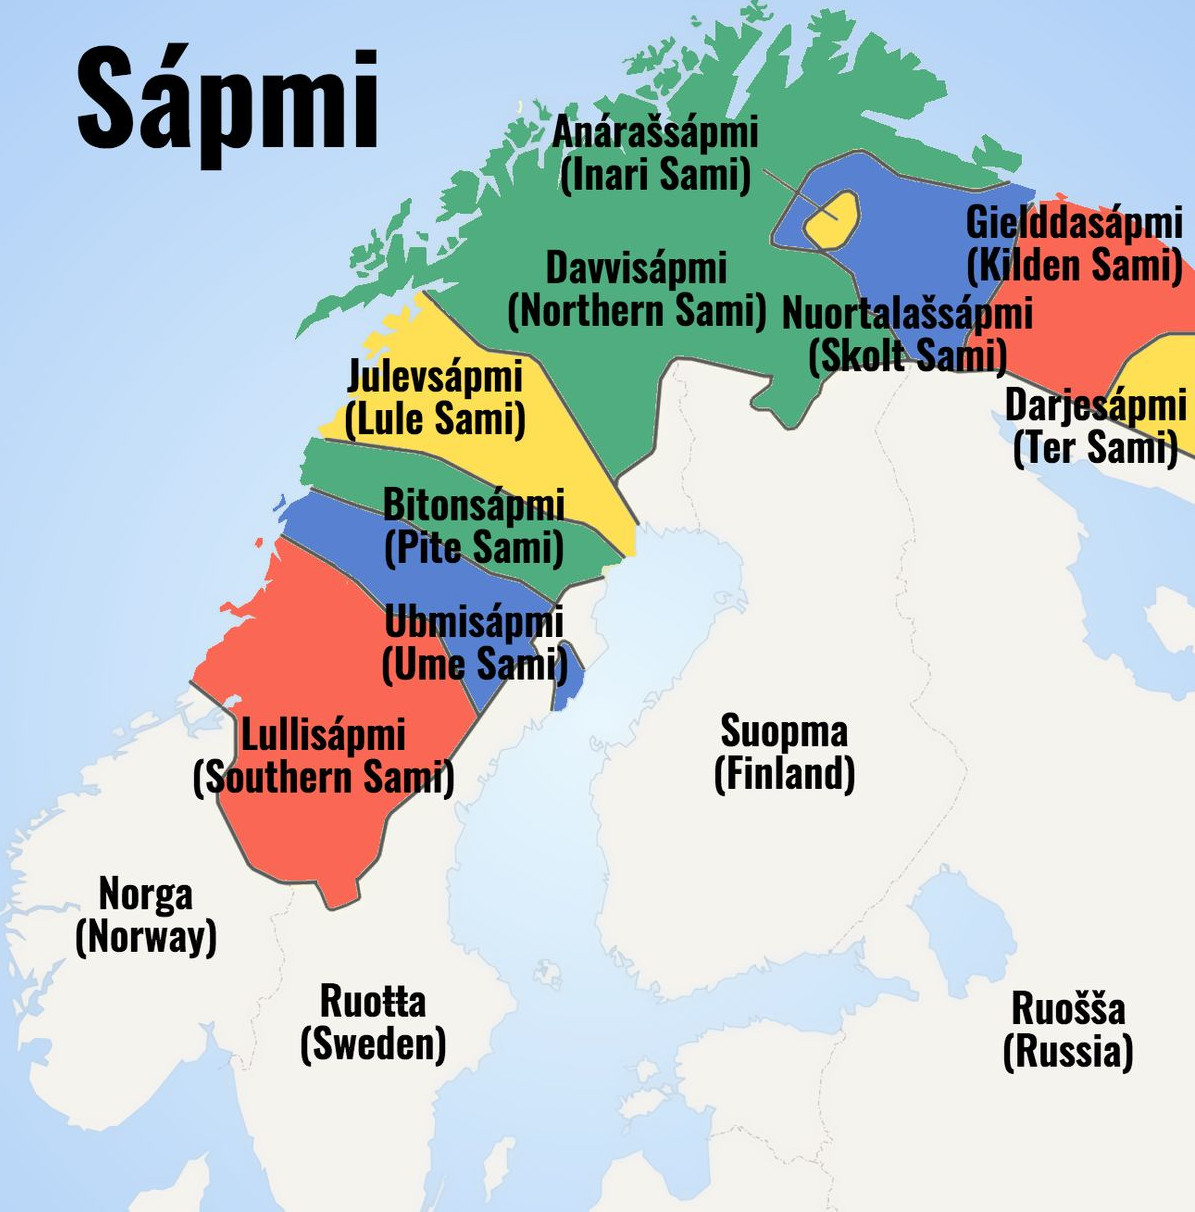
\includegraphics[width=\linewidth]{figures/sapmi1.jpg}
  \caption{The S\'{a}pmi region, spanning the northern parts of Norway, Sweden, Finland and Russia, with the geographic distribution of the nine spoken S\'{a}mi varieties. North S\'{a}mi (\textit{Davvis\'{a}pmi}) covers the largest area. Source: The Decolonial Atlas~\cite{decolonialatlas}, reused under the Decolonial Media License 0.1.}
\label{fig:sapmi-map}
\end{figure}

There are nine mutually unintelligible spoken S\'{a}mi varieties across the S\'{a}pmi region~\cite{sammallahti1998}. The most widely spoken variety, and the focus of this project given the data and tooling available, is North S\'{a}mi (\texttt{ISO 639-3 sme}, \textit{Davvis\'{a}megiella}), with around \smiSpeakers{} speakers, while the most endangered varieties have fewer than 50 speakers, and some are no longer actively spoken~\cite{moseley2010,sammallahti1998}. The S\'{a}mi languages belong to the Uralic family, which also includes Finnish, Estonian and Hungarian~\cite{sammallahti1998}. According to UNESCO's \textit{Atlas of the World's Languages in Danger}~\cite{moseley2010}, North S\'{a}mi is classified as \textit{definitely endangered} (children no longer learn the language as a mother tongue in the home), while the more endangered varieties (Pite, Ter, Ume) are classified as \textit{critically endangered} (the youngest speakers are grandparents and older, who use the language partially and infrequently).

\section{Linguistic Characteristics of North S\'{a}mi}

North S\'{a}mi is an
agglutinative\footnote{
Agglutinative languages build words by stacking distinct morphemes onto a stem, with each suffix typically carrying a single grammatical meaning. For example, North S\'{a}mi \textit{viesuiguin} ``with the houses'' decomposes as \textit{viesu-} (`house') + \textit{-i-} (plural) + \textit{-guin} (`with', the comitative case).}
language with complex morphology and hundreds of inflected\footnote{ Inflection refers to systematic modifications of a word that mark grammatical categories such as case, number, tense, or person. North S\'{a}mi nouns inflect for six cases in singular and plural, while pronouns and verbs additionally distinguish a dual number, yielding many distinct surface forms per stem.}
forms per verb~\cite{valijarvi2013}.
This agglutinative morphology yields large type token ratios even in modest corpora: meaning that the OCR model rarely sees the same exact word twice during training, so it cannot memorise word shapes altogether and is forced to learn the script at the character level. The orthography of North S\'{a}mi further complicates this by including seven special characters (diacritics and modified letters: \'{a}, \v{c}, đ, ŋ, \v{s}, ŧ, \v{z}) that distinguish it from the standard Latin script~\cite{valijarvi2013}.


It also possesses a three way quantity contrast. There are three consonant lengths (short, long, and overlong), and the difference between these lengths carries a grammatical meaning. In writing, only a part of this is captured: long and overlong consonants are both spelled the same way, as a doubled letter, and the two are told apart only in specialized linguistic notation~\cite{valijarvi2013}.

The length difference, in North S\'{a}mi, between single and doubled consonants, does grammatical work through a process called consonant gradation. For example, the noun \textit{giella} ``language'' is spelled with a double \textit{ll}, but in a possessive form, \textit{giela} has only a single \textit{l}~\cite{valijarvi2013}. In other words, that single letter is the only thing marking the difference between the two grammatical forms. If an OCR system drops or misreads one character, it can change the grammatical meaning of the word entirely. This is why getting individual characters right matters so much for the NLP tasks that follow.


Before 1979, the three Nordic countries used separate standardised orthographies for North S\'{a}mi, and a unified orthography was only adopted that year (last revised in 1985)~\cite{valijarvi2013}. Many historical documents are therefore written in previous conventions, adding a further layer of complexity for OCR models, which must generalise across orthographic registers to be effective for heritage digitisation. For example, Turi's \textit{Muittalus Samid Birra} (1910)\cite{turi1910}\footnote{In standard modern North S\'{a}mi orthography this title is written \textit{Muitalus s\'{a}miid birra} (the form used elsewhere in this report). The spelling here preserves Turi's original 1910 Friis orthography to illustrate the early conventions.} uses the Friis orthography. "An Account of Sami" (eng), is the first secular book released in North S\'{a}mi, tells about the life of people herding reindeer in the Jukkasjärvi region of northern Sweden at the beginning of the 20th century, and is included in the out of distribution evaluation set to test the model's ability to generalise across orthographic conventions.

\begin{figure}[h]
\centering

\includegraphics[width=0.85\linewidth]{figures/combined_example.pdf}
\caption{The seven special diacritical characters that distinguish North S\'{a}mi orthography from the standard Latin script. For each character, an example word is shown that uses it. The visual similarity between several pairs (e.g.\ \v{c}/c, \v{s}/s, \v{z}/z, ŧ/t) makes their reliable recognition one of the central technical challenges for an OCR model trained on this script.}
\label{fig:report-alphabet}
\end{figure}

\section{Personal Motivation}
\label{sec:personal-motivation}

I chose this topic because I find it personally meaningful to work on a project that has the potential to contribute to the preservation of endangered languages. I think that the democratization of technology is an important matter in modern life. Even in resource constrained settings, the same tools should be available to everyone, and that includes the tools for digitizing and preserving cultural heritage. Additionally, I was intrigued by the technical challenges in OCR for low resource languages, and I wanted to explore how machine learning techniques could be adapted to work effectively in such contexts. Lastly, I come from a region situated in southern Poland, where the Silesian language is spoken, which is also a low resource language. This personal connection further motivated me to contribute to this field of research.


\section{Technical Context}
\label{sec:technical-context}

The project uses Python 3.11. The whole development environment, system libraries and CUDA driver are declared in a single \texttt{flake.nix} using Nix flakes\footnote{Nix flakes, \url{https://nix.dev/concepts/flakes}.}.
Entering the shell with \texttt{nix develop} provides an identical environment on both the local development laptop and the uCloud GPU node, with Python dependencies pinned via \texttt{requirements.txt} (captured by \texttt{pip freeze} inside the flake shell for full reproducibility).

The machine learning stack is built on PyTorch~2.11~\cite{paszke2019pytorch} with \texttt{torchvision} for the ImageNet pretrained backbones and CUDA~13 with cuDNN for GPU acceleration. 
The Hugging Face ecosystem provides the supporting infrastructure: \texttt{datasets}~\cite{lhoest2021datasets} streams the Spr\r{a}kbanken North S\'{a}mi OCR corpus directly from the Hub, and \texttt{safetensors} handles model checkpoint serialisation.

Image preprocessing relies on \texttt{opencv-python} and \texttt{pillow}, while the \texttt{pdfminer} and NLTK power the PDF parsing and sentence segmentation used by the alignment TUI tool.

Evaluation uses community standard implementations: \texttt{jiwer} for character and word error rates (CER, WER) on the OCR side, and \texttt{sacrebleu}~\cite{post2018call} for BLEU on the translation side, ensuring the reported scores follow the same definitions used in the literature. Supporting analysis and visualisation is done with \texttt{numpy}, \texttt{pandas}, \texttt{scikit-learn}, \texttt{matplotlib}, \texttt{seaborn} and \texttt{wordcloud}, with exploratory work hosted in Jupyter notebooks.

Compute is run on NVIDIA Tesla V100 32GB on uCloud (SDU/DeiC) for training and a development AMD Ryzen 5 PRO laptop CPU for the inference benchmark, purposefully chosen to reflect a realistic low resource deployment environment rather than ideal serving hardware.



% Goals in 'chap-goals.tex'
\chapter{Goals}
\label{chap:goals}

While there are some rule based systems for North S\'{a}mi in place, such as those provided by Giellatekno~\cite{giellatekno}, including morphological analysers, dictionaries, grammar parsers and single language corpora. In other digitalisation sectors the S\'{a}mi languages remain underrepresented, which is itself a barrier to heritage digitisation and language revitalisation efforts~\cite{enstad2025}.
The most accurate publicly available OCR models for North S\'{a}mi are transformer based variants fine tuned by the National Library of Norway on synthetic data and released through the Spr\r{a}kbanken S\'{a}mi OCR collection~\cite{enstad2025,sprakbanken_collection}. However, these models are computationally heavy. They take \trocrInferenceIntroSec{}+ seconds per image on a CPU and around \trocrSize{}~MB of storage memory, which makes them impractical for community driven projects, mobile field documentation, and institutions with limited infrastructure. As shown in Figure~\ref{fig:report-design-space}, there is a clear gap in the design space for models that balance accuracy with deployability, particularly for low resource languages like North S\'{a}mi.

\begin{figure}
    \centering
    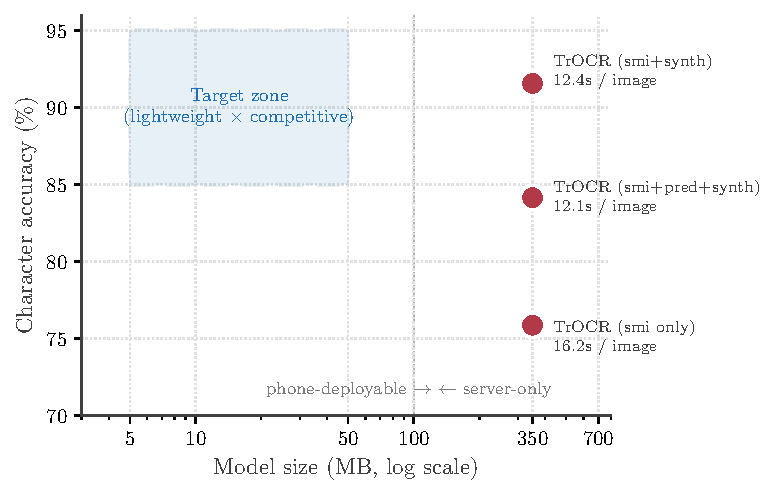
\includegraphics[width=0.8\textwidth]{figures/design_space.pdf}
    \caption{Design space of North S\'{a}mi OCR models, plotting accuracy against model size (MB) and inference time (seconds). Existing transformer based models cluster in the high accuracy but large size region, while the proposed lightweight CNN-CTC model aims for a target zone of competitive accuracy with significantly reduced size and inference time.}
    \label{fig:report-design-space}
\end{figure}

This project aims to explore whether a lightweight OCR can achieve a high accuracy for North S\'{a}mi while allowing practical deployability.
Additionally, the project tests the out of domain robustness of such lightweight models on historical lexical content, which is crucial for heritage digitisation, and verifies its feasibility as a component in an end to end OCR$\rightarrow$MT pipeline for smart learning and archival indexing use cases. After analysing the benchmarking results, further conjunction based sentence splitting is proposed as a linguistically motivated preprocessing step to mitigate the fixed width input penalty of the lightweight architecture, showing that architectural and linguistic adaptations can work together to improve performance under deployment constraints.

\section{Research Question}
\label{sec:research-question}
The main research question guiding this project is: 

\begin{quote}
\textit{Can a lightweight OCR architecture approach Transformer level accuracy for North S\'{a}mi while enabling practical deployment on modest hardware?}.
\end{quote}

The emphasis on deployment constraints is a crucial aspect of the project, as it looks into one of the often overlooked parts of research: the practicality and usability of the proposed solutions. The project doesn't focus solely on accuracy, but also looks at ways of mitigating some technological constraints given by the hardware and resource limitations.

\section{Specific Goals}
\label{sec:contributions}

As listed in the scientific article, the six main contributions of this project are: 


\begin{enumerate}
    \item A lightweight CNN-CTC architecture for North S\'{a}mi OCR, achieving a competitive balance of accuracy and deployability.
    \item A systematic benchmark comparing the proposed model against 7 TrOCR variants and 3 CTC variants with ImageNet pretrained backbones, demonstrating the tradeoffs between accuracy and computational efficiency.
    \item A contribution to Sustainable AI through a lightweight CNN-CTC model.
    \item A linguistically motivated conjunction based sentence splitting method that mitigates the fixed width input penalty of lightweight architectures, improving long sentence accuracy under oracle ground truth conditions, as a proof of concept.
    \item An end to end OCR$\rightarrow$MT pipeline integrating the proposed model with TartuNLP's North Sámi English API, demonstrating usability for downstream tasks.
    \item Demonstrating usefulness in 21st century education, AI \& NLP, and next generation robotic systems applied to low resource languages.
\end{enumerate}

% \begin{enumerate}
%     \item \textbf{A lightweight CNN--CTC architecture} for North S\'{a}mi OCR that achieves a competitive accuracy/deployability balance: \ctcCharAcc{}\% character accuracy in \ctcSize{}~MB on disk and \ctcTime{}~s per image on CPU (Section~\ref{sec:main-result}).
%     \item \textbf{A systematic benchmark} comparing the proposed model against 7 TrOCR variants and 3 CTC variants with ImageNet-pretrained backbones, on a shared \testSamples{}-sample test set and a single CPU, isolating the accuracy--efficiency trade-off (Section~\ref{sec:main-result}).
%     \item \textbf{A contribution to Sustainable AI} through the lightweight CNN--CTC model, running roughly \speedupFactor{}$\times$ faster and at \sizeRatio{}$\times$ smaller size than the strongest TrOCR baseline --- translating to a million-page corpus processable in under \millionPagesCtcHours{}~hours on CPU rather than $\sim$\millionPagesTrocrDays{}~days (Section~\ref{sec:main-result}).
%     \item \textbf{An end-to-end OCR$\rightarrow$MT pipeline} integrating the proposed model with TartuNLP's North~S\'{a}mi--English machine-translation API~\cite{tartunlp}, scored on a parallel out-of-domain set with BLEU, chrF and TER (Section~\ref{sec:e2e}).
%     \item \textbf{A linguistically-motivated conjunction-based sentence splitting method} that mitigates the fixed-width input penalty of lightweight architectures, dropping long-sentence CER from \splitLongOriginalCER{}\% to \splitLongSplitCER{}\% (paired test $p = \splitPValue{}$, Cohen's $d = \splitCohensD{}$; Section~\ref{sec:conjunction-split}).
%     \item \textbf{Demonstrating usefulness in 21st-century education, AI \& NLP and next-generation robotic systems} applied to low-resource languages --- the deployability profile (\ctcSize{}~MB / sub-100~ms) makes the model a candidate for mobile heritage-preservation apps, archival indexing, classroom tooling and joint OCR + reconstruction in everyday-vision settings (Section~\ref{sec:applications}).
% \end{enumerate}

% Process desc in 'chap-process.tex' 
\chapter{Process}
\label{chap:process}

\noindent\textit{Readers without an ML/AI background may find the brief explanation of concepts from this chapter in Appendix~\ref{appendix:concepts}.}

\section{Dataset Exploration}

First, the Spr\r{a}kbanken S\'{a}mi OCR corpus~\cite{sprakbanken_dataset,enstad2025} from Hugging Face was analysed. It consists of train/validation/test splits (307k/40.8k/84.5k rows), ment for fitting OCR models for North S\'{a}mi, Lule and Inari S\'{a}mi. Each sample is a single synthetically rendered text line paired with its ground truth transcription, e.g.\ those shown in Figure~\ref{fig:report-samples}. The line by line format meant that line detection and layout analysis were outside the scope of the model. The OCR goal was to transcribe the line of text into a string.
Extracted vocabulary yielded a \charsetSize{} symbol charset (\numCharsVocab{} characters plus one CTC blank token) later used by the CTC head. The computed word and letter frequencies are rendered as the clouds in Figure~\ref{fig:report-corpus}. 
Two observations from this step shaped later decisions. The conjunction \textit{ja} (``and'') dominates the word distribution, foreshadowing the conjunction splitting preprocessing. The seven special characters appear at non-negligible frequencies.

\begin{figure}[h]
\centering
\begin{tabular}{c}

\includegraphics[width=0.92\linewidth]{figures/correct2.jpg} \\[2pt]
\footnotesize \textit{mij\'{a}v juohkkal\'{a}hk\'{a}j kreatijvvan.} \\[10pt]

\includegraphics[width=0.92\linewidth]{figures/example1.jpg} \\[2pt]
\footnotesize \textit{sámi vuoigatvuođalaččaiguin, guoskevaš oasálaččaiguin} \\
\end{tabular}
\caption{Two Spr\r{a}kbanken synthetic samples shown as the model sees them.The rendering varies font, spacing, slight noise and background to simulate scanned text appearance.}
\label{fig:report-samples}
\end{figure}

\begin{figure}[h]
\centering
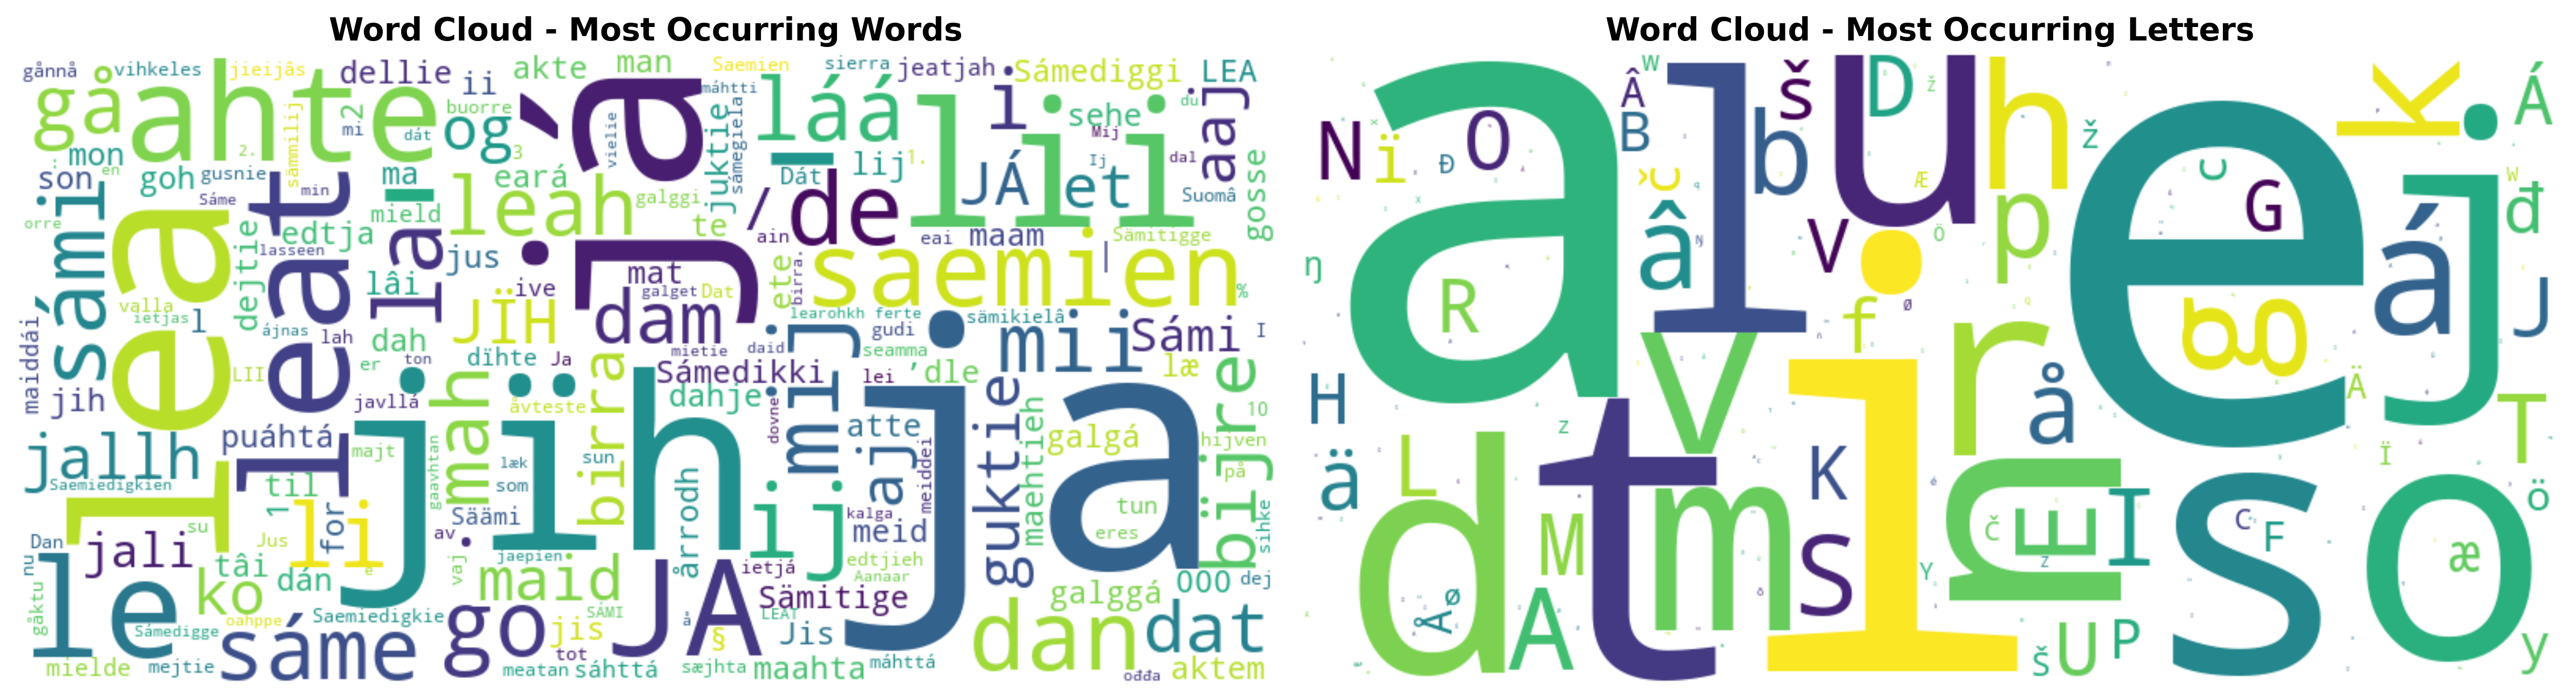
\includegraphics[width=\linewidth]{figures/word_letter_clouds.png}
\caption{Word and letter clouds of the Spr\r{a}kbanken North S\'{a}mi training corpus.}
\label{fig:report-corpus}
\end{figure}

\section{Corpus Building Detour}
\label{sec:corpus-detour}

A small detour was taken during the early stages of the project to assess whether a parallel English S\'{a}mi corpus could be built from Turi's \textit{Muitalus s\'{a}miid birra} (1910). The idea was to explore a possibility of training a MT solution using the yielded corpora (e.g. Gated Recurrent Unit (GRU) Network) Both versions of the book were obtained as PDFs, one in North S\'{a}mi (Friis' orthography), the other in English (translated and edited by Thomas A. DuBois), alongside an already parsed, sentence split S\'{a}mi version from the Giellatekno website.

The PDFs are parsed with \texttt{pdfminer}, split into sentences with NLTK, and aligned with a custom TUI tool that supports manual approval (See Figure~\ref{fig:alignment-tool}), deletion, and merging of sentence pairs. Due to time constraints, the tool was ultimately not used to generate a full bilingual corpus, instead, it produced a small evaluation set of \bookTestSamples{} synthetic renderings of the S\'{a}mi sentences, which became the out of domain test set in the IISA paper.

\begin{figure}[h]
\centering
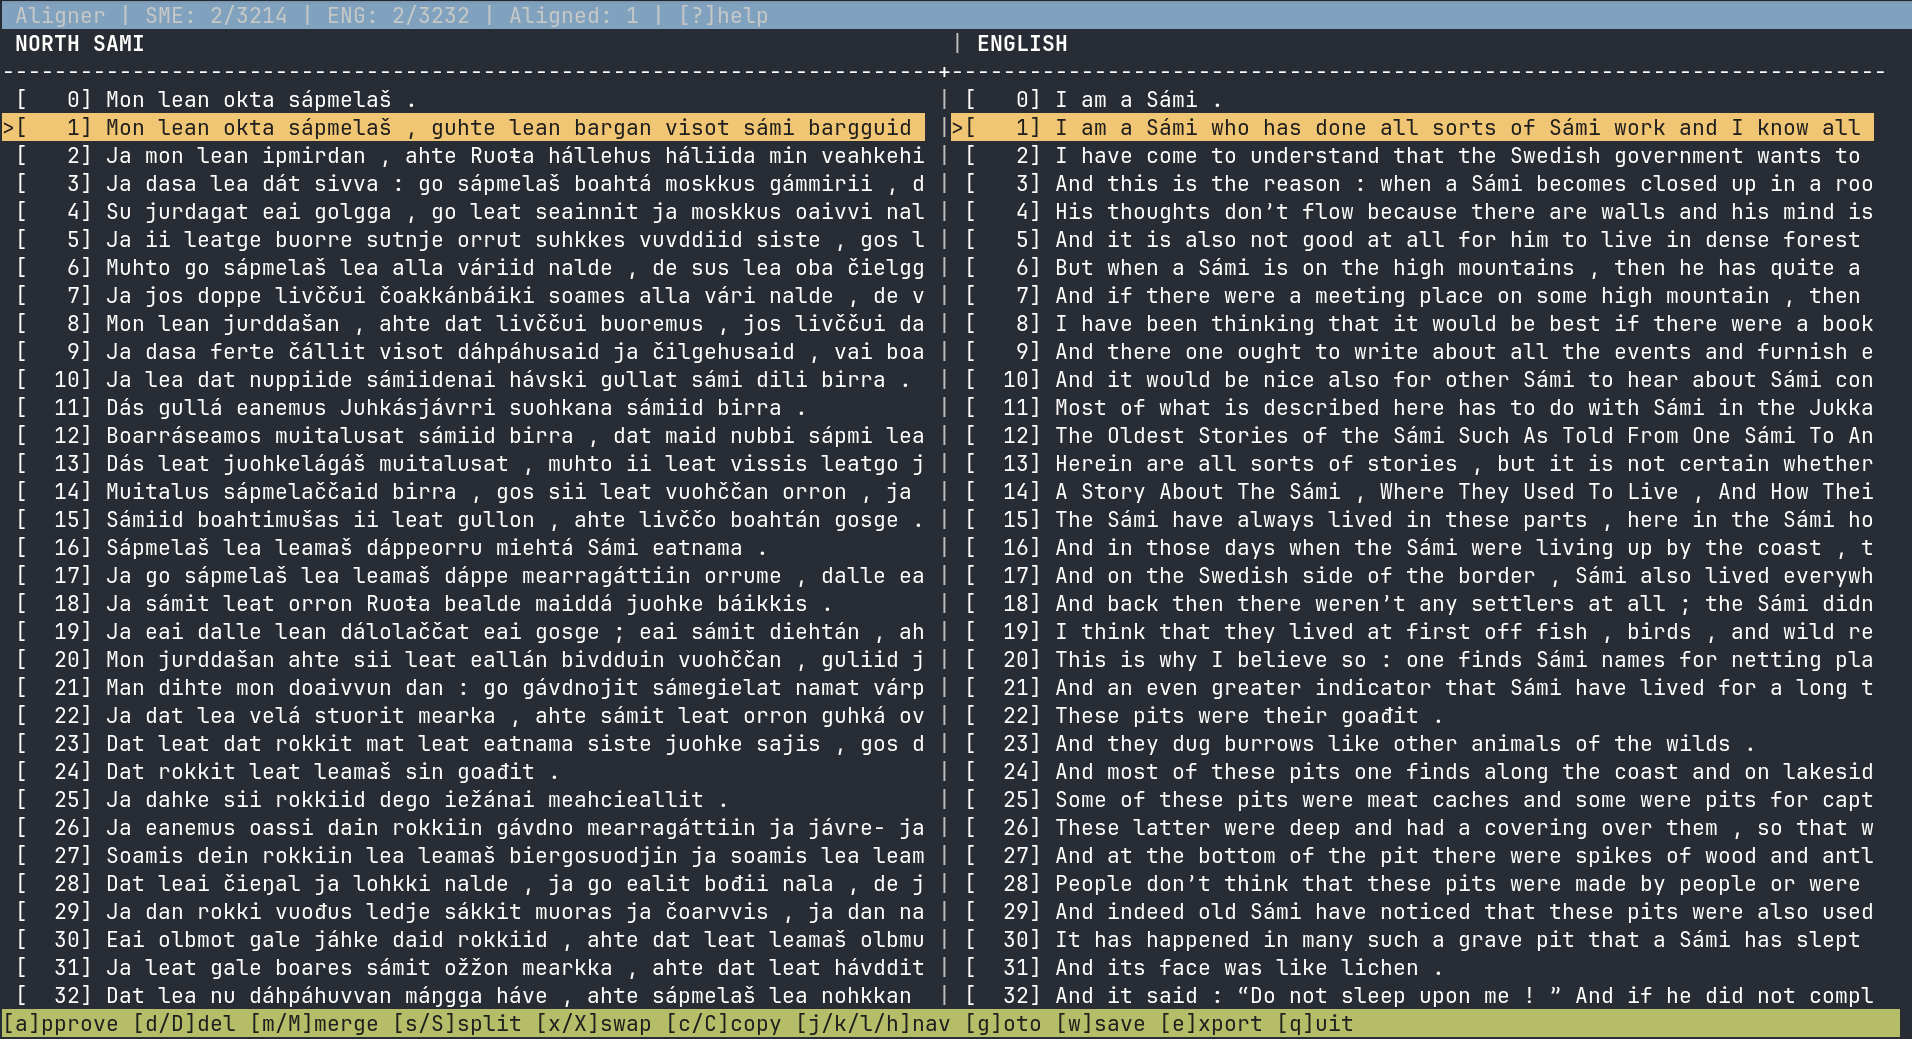
\includegraphics[width=\linewidth]{figures/alignment-tool.png}
\caption{Alignment CLI tool for parallel corpora generation from two sources.}
\label{fig:alignment-tool}
\end{figure}

\section{Training Pipeline Overview}
\label{sec:pipeline-overview}

The modular OCR pipeline consists of three slots: a \emph{backbone}, an \emph{encoder} and a \emph{decoder}. Each slot is easily swappable, yielding 15 distinct configurations in total: 5 backbones (SimpleCNN, VGG16, VGG19, ResNet50, ResNet101) $\times$ 3 encoders (none, BiLSTM, Transformer), with a fixed CTC decoder across all variants. A training queue runs configurations consecutively without manual intervention, logging each step and storing checkpoints and outputs in a structured way for monitoring and debugging. The modular design also leaves room for future extensions, such as a post correction module or a scan quality classifier.

This layout is inspired by Shi et al.'s CRNN~\cite{shi2017crnn}: a CNN backbone extracts spatial features, a sequence encoder adds temporal context, and a CTC head maps the encoded sequence to characters. Each component is explained in more detail below.

\subsection{Backbone}
\label{subsec:backbone}

The backbone slot contains the CNN feature extractor, which processes the input image into a sequence of column features. The proposed lightweight variant is a 7 layer SimpleCNN trained from scratch, while the comparison variants use ImageNet pretrained VGG16, VGG19, ResNet50 and ResNet101 backbones with differential learning rates to preserve pretrained features.

\subsection{Encoder}
\label{subsec:encoder}

The encoder slot contains the sequence modelling component, which captures contextual dependencies between characters. The options are a 2 layer BiLSTM, a Transformer encoder block, or no encoder (direct CNN to CTC). This allowed to isolate the contribution of explicit sequence modelling on top of the per column CNN features.

\subsection{Decoder}
\label{subsec:decoder}

The decoder slot contains the transcription head, which maps the encoded features to character probabilities. A CTC decoder \cite{graves2006ctc} is used across all configurations, which allows for training without explicit character level alignment and handles variable length outputs. This fixed decoder setup ensures that differences in performance can be attributed to the backbone and encoder choices.

\section{Comparison}
\label{sec:comparison}

The modular pipeline allowed for a systematic comparison of the CNN based variants against the transformer based models. The comparison benchmark was run on CPU to reflect realistic deployment conditions, and evaluated on the same test set using consistent metrics (CER, WER, exact match accuracy).

Due to limited accessibility to uCloud resources only the following variants were trained: \texttt{ctc\_simple} (the lightweight 7 layer SimpleCNN trained from scratch), \texttt{ctc\_vgg16} and \texttt{ctc\_vgg19} (ImageNet pretrained VGG backbones with differential learning rates), and \texttt{ctc\_resnet50} (ImageNet pretrained ResNet50). The \texttt{ctc\_resnet101} variant was gated on the ResNet50 results. Per epoch time on the V100 was $\sim$19~minutes for the VGG pair and $\sim$76~minutes for ResNet50, so a full 100 epoch run would have occupied the GPU for $\sim$32~hours (VGG) or $\sim$5~days (ResNet50). 
In practice all three pretrained variants triggered early stopping well before that: \texttt{ctc\_vgg16} at 52~epochs, \texttt{ctc\_vgg19} at 63~epochs, and \texttt{ctc\_resnet50} at 37~epochs ($\sim$48~hours), with validation CER stuck around 0.69 to 0.73 at early stopping (ResNet50's final test CER of 0.753 reflects continued degradation past that point, see Section~\ref{sec:main-result}). The compute budget made it impossible to commit further.

\section{The lightweight CNN-CTC variant}
\label{sec:lightweight-backbone}

The headline lightweight variant, \texttt{ctc\_simple}, uses a 7 layer SimpleCNN backbone trained from scratch, no encoder and a CTC head over the \charsetSize{} symbol vocabulary. The architecture is shown in Figure~\ref{fig:report-architecture}.

\begin{figure}[h]
\centering

\includegraphics[width=\linewidth, height=0.8\textheight, keepaspectratio]{figures/architecture_tikz.pdf}
\caption{Modular OCR pipeline used in the IISA paper. The lightweight \texttt{ctc\_simple} variant uses a 7 layer SimpleCNN backbone trained from scratch and a CTC head over the \charsetSize{} symbol vocabulary, the encoder slot is left empty.}
\label{fig:report-architecture}
\end{figure}

The SimpleCNN has 7 convolutional layers with following channel widths $64, 128, 256, 256, 512, 512, 512$, each followed by batch normalisation and a ReLU activation function.
Pooling is asymmetric: $2\times 2$ max pooling in the early layers progressively collapses both axes, while the later layers switch to $2\times 1$ pooling that keeps horizontal resolution intact, preserving the character ordering that the CTC head relies on. A final adaptive pool reduces feature map height to 1, yielding a sequence of column vectors. These are projected to \hiddenDim{} dimensions and passed directly to a linear head that maps to \charsetSize{} classes (\numCharsVocab{} characters plus the CTC blank) followed by LogSoftmax.
The full model has $\sim$\numParams{}M parameters.
It is trained with a CTC loss that marginalises over all valid character alignments and decoded greedily at inference time.
In practice it ran the full 100 epoch schedule at $\sim$8 minutes per epoch ($\sim$13 hours).


\section{Training Setup}
\label{sec:training-setup}

All CTC variants share the same training recipe with backbone specific overrides. The optimiser is AdamW with a base learning rate of $10^{-4}$ and weight decay $10^{-4}$ for \texttt{ctc\_simple}, reduced to $3\times 10^{-5}$ with a 0.1$\times$ differential multiplier on pretrained VGG and ResNet50 layers. The batch size is 32 for SimpleCNN and VGG, reduced to 16 for ResNet50 due to GPU memory. Training runs for up to 100 epochs with early stopping (patience 15 to 35 epochs, scaling with model size), \texttt{ReduceLROnPlateau} halves the learning rate when validation CER plateaus, and gradients are clipped to a max norm of 5.0 to stabilise the CTC loss.

The training data is the Spr\r{a}kbanken synthetic North S\'{a}mi OCR corpus~\cite{sprakbanken_dataset,enstad2025}, with \trainSamples{} samples in the training subset (90\% of the 307{,}387-sample training split) and roughly \hfValidationSamples{} held out for development. 


\section{Evaluation and End to End Pipeline}
\label{sec:evaluation-pipeline}

Evaluation is conducted on a \testSamples{} sample combined test set: \hfTestSamples{} held out samples from the Spr\r{a}kbanken validation split (in domain) and \bookTestSamples{} synthetic renderings of Turi's \turiYear{} \textit{Muitalus s\'{a}miid birra} (out of domain lexical content). Models are scored with character error rate (CER), word error rate (WER), exact match accuracy, and a normalised accuracy variant that removes punctuation and extra whitespaces, all computed as Levenshtein distance on raw UTF-8 strings. Per image inference time is measured on CPU to reflect realistic deployment conditions. The TrOCR variants are used as released by the National Library of Norway without additional fine tuning, while \texttt{ctc\_simple} is trained from scratch on the Spr\r{a}kbanken corpus. The benchmark compares a ready pretrained baseline against a purpose trained lightweight model.

The full end to end pipeline passes the OCR predictions into the TartuNLP North S\'{a}mi English machine translation API~\cite{tartunlp}, with the translated output scored against the English reference using BLEU, chrF~\cite{popovic2015chrf}, and TER (See Figure~\ref{fig:ocr-mt-pipeline}).

\section{Conjunction Splitting Experiment}
\label{sec:conjunction-split-process}

The experiment surfaced from the benchmark results. Per sentence error analysis on both \texttt{ctc\_simple} and the strongest TrOCR variants showed a steep accuracy drop beyond roughly \sentenceLengthThreshold{} characters, caused by the fixed \preprocessingImgWidth{} px input width cutoff. Referencing the most frequently used words in the dataset (Figure~\ref{fig:report-topwords})  where the conjunction \textit{ja} dominated the distribution suggested that splitting long inputs at North S\'{a}mi conjunction boundaries (\textit{ja} ``and'', \textit{muhto} ``but'', \textit{dahje} ``or'', \textit{go} ``when/because'', \textit{ahte} ``that'', \textit{jos} ``if'') before OCR and rejoin the predictions afterwards, might mitigate that issue.

\begin{figure}[h]
\centering
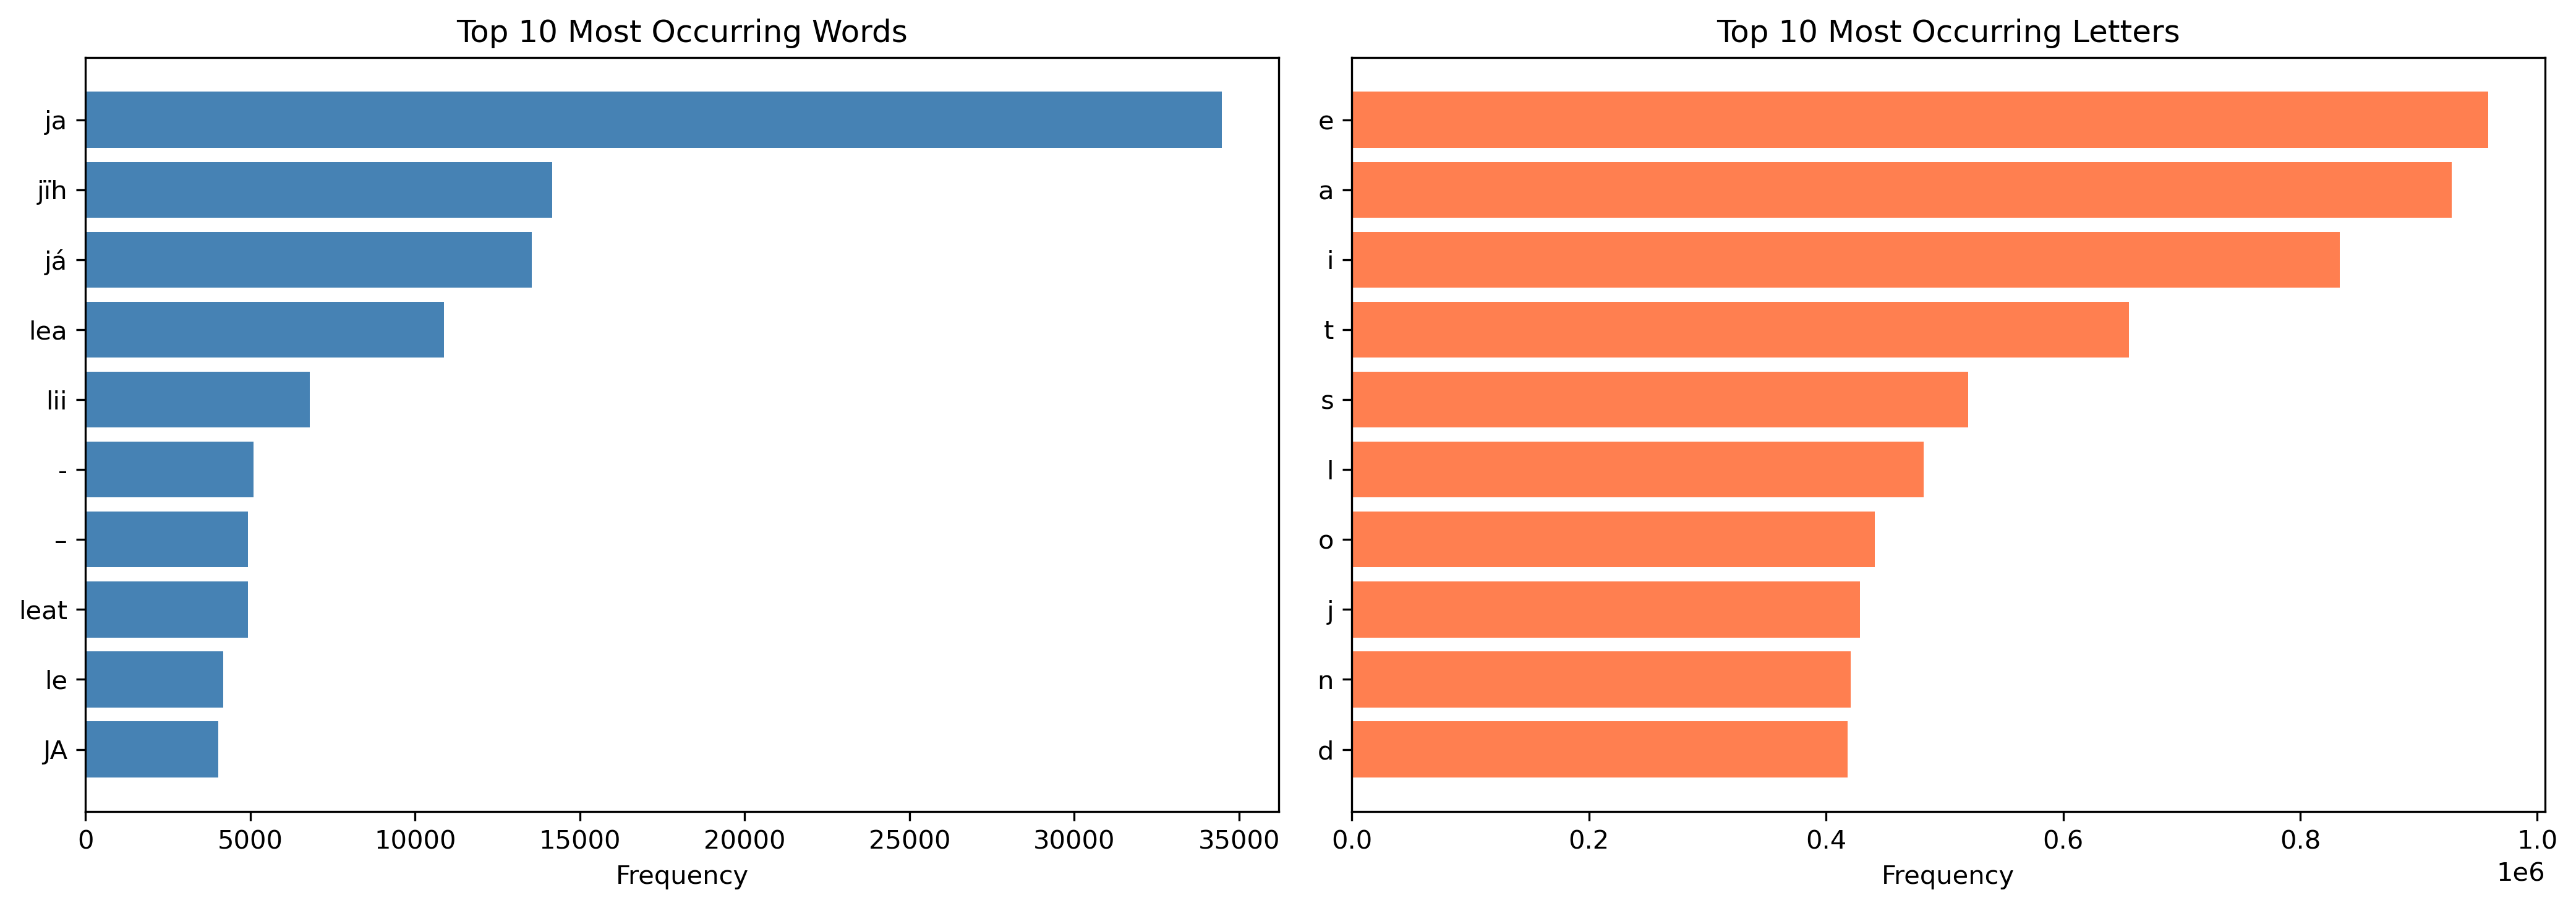
\includegraphics[width=\linewidth]{figures/top_words_letters_bars.png}
\caption{Top 10 most frequent words (left) and characters (right) in the Spr\r{a}kbanken North S\'{a}mi training corpus. The conjunction \textit{ja} (``and'') is by far the most frequent token, motivating conjunction based segmentation.}
\label{fig:report-topwords}
\end{figure}

More specifically, every input sentence longer than \sentenceLengthThreshold{} characters is scanned for these conjunction tokens by a case insensitive word boundary regex matching (the implementation also extends to multi-word and subordinate variants such as \textit{ovdal go} ``before'' and \textit{dasgo} ``because''), with the multi-word forms being matched greedily before their single-word counterparts to avoid double counting. The text is split immediately \textit{before} each matched conjunction so the connective stays attached to its following clause, and a minimum segment length of 20 characters guards against over splitting when there are many conjunctions close to eachother. Each resulting text segment is then re-rendered as a fresh synthetic line image through the same generator used for the evaluation out-of-domain data, passed independently through \texttt{ctc\_simple}, and the per segment predictions are joined with single space to form the final transcription. The benchmark compares per sample CER on the long sentence subset of the test set before and after splitting, with statistical significance estimated via a paired test and effect size reported as Cohen's $d$.

\begin{figure}[h]
\centering
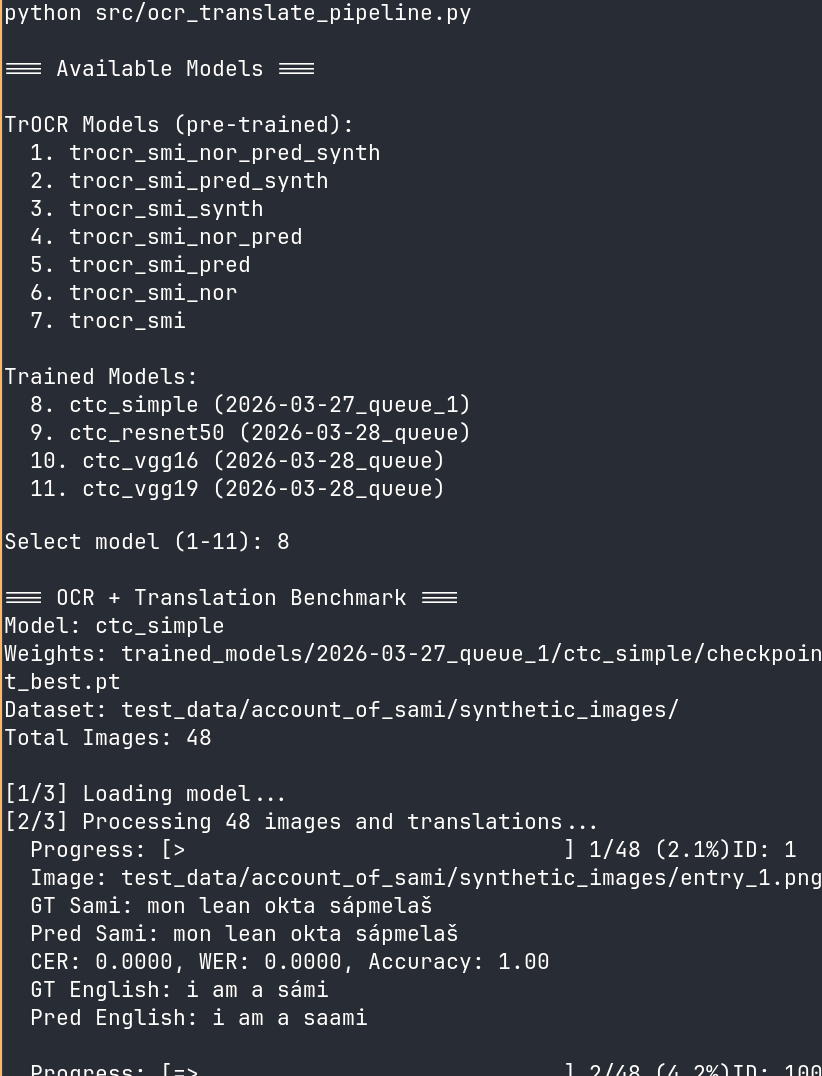
\includegraphics[width=\linewidth]{figures/ocr-mt-pipeline.png}
\caption{CLI tool for running the end to end OCR$\rightarrow$translation pipeline. The user selects the OCR model and dataset, and the tool reports both OCR accuracy metrics (CER, WER) and translation quality metrics (BLEU, chrF, TER) on the translated output.}
\label{fig:ocr-mt-pipeline}
\end{figure}

% Reflections chapter in 'chap-process-reflections.tex'
\chapter{Process Reflections}
\label{chap:process-reflections}

\section{Main Results}
\label{sec:main-result}

The headline benchmark from the scientific article compares the proposed \texttt{ctc\_simple} against the National Library of Norway's best TrOCR variants. The strongest TrOCR variant (\texttt{trocr\_smi\_synth}) sets the SOTA at \trocrBestCER{}\% CER (\trocrBestCharAcc{}\% character accuracy\footnote{Character accuracy is measured directly and does not equal $100-\text{CER}$, since CER counts insertions as well as substitutions and deletions.}), with \texttt{ctc\_simple} within \cerGap{}~pp at \ctcCER{}\% CER (\ctcCharAcc{}\% character accuracy). On efficiency the picture flips. The lightweight model runs roughly \speedupFactor{}$\times$ faster on the same CPU and is \sizeRatio{}$\times$ smaller (\ctcSize{}~MB vs.\ \trocrSize{}~MB), which is decisive for heritage digitisation. At \ctcTime{}~s per image a CPU pushes about \ctcThroughputK{},000 images per hour, so a million page corpus runs in under \millionPagesCtcHours{} hours where TrOCR would need around \millionPagesTrocrDays{} days, and the small footprint fits edge devices that TrOCR cannot.

Table~\ref{tab:extended_results} reports the complete benchmark across all 11 models: the seven TrOCR variants released by the National Library of Norway, the proposed \texttt{ctc\_simple}, and the three ImageNet-pretrained CTC backbones that failed to converge. Extended comparison plot from the scientific article in Figure~\ref{fig:comparison1}.

\begin{table}[h]
\centering
\caption{OCR benchmark on \testSamples{} test samples: all 7 TrOCR variants from the National Library of Norway, the proposed lightweight \texttt{ctc\_simple}, and the three ImageNet-pretrained CTC backbones that failed to converge. Bold marks the best value in each column. Lower CER/WER is better, higher Exact Match Accuracy is better.}
\label{tab:extended_results}
\small
\resizebox{\linewidth}{!}{%
\begin{tabular}{@{}llccccc@{}}
\toprule
\textbf{Model} & \textbf{Training Data} & \textbf{CER↓} & \textbf{WER↓} & \textbf{Exact↑} & \textbf{sec / img} & \textbf{Size} \\
 & & \textbf{(\%)} & \textbf{(\%)} & \textbf{(\%)} & & \textbf{(MB)} \\
\midrule
trocr\_smi\_synth & Smi+Synth & \textbf{\trocrBestCER{}} & \textbf{\trocrBestWER{}} & \textbf{42.08} & \trocrBestTime{} & $\sim$\trocrSize{} \\
\textbf{ctc\_simple} & Smi+Synth & \ctcCER{} & \ctcWER{} & 36.74 & \textbf{\ctcTime{}} & \textbf{\ctcSize{}} \\
trocr\_smi\_pred\_synth & Smi+Pred+Synth & \trocrSmiPredSynthCER{} & \trocrSmiPredSynthWER{} & \trocrSmiPredSynthWordAcc{} & \trocrSmiPredSynthTime{} & $\sim$\trocrSize{} \\
trocr\_smi\_nor\_pred\_synth & Smi+Nor+Pred+Synth & \trocrSmiNorPredSynthCER{} & \trocrSmiNorPredSynthWER{} & \trocrSmiNorPredSynthWordAcc{} & \trocrSmiNorPredSynthTime{} & $\sim$\trocrSize{} \\
trocr\_smi & Smi only & \trocrSmiCER{} & \trocrSmiWER{} & \trocrSmiWordAcc{} & \trocrSmiTime{} & $\sim$\trocrSize{} \\
trocr\_smi\_pred & Smi+Pred & 24.82 & 63.06 & 16.32 & 11.730 & $\sim$350 \\
trocr\_smi\_nor & Smi+Nor & 25.84 & 66.62 & 13.17 & 12.890 & $\sim$350 \\
trocr\_smi\_nor\_pred & Smi+Nor+Pred & 26.43 & 64.21 & 17.08 & 11.759 & $\sim$350 \\
ctc\_vgg19 & Smi+Synth & 71.86 & 97.89 & 0.00 & 0.055 & $\sim$550 \\
ctc\_vgg16 & Smi+Synth & 73.94 & 98.81 & 0.00 & 0.044 & $\sim$550 \\
ctc\_resnet50 & Smi+Synth & 75.30 & 98.64 & 0.00 & 0.034 & $\sim$100 \\
\bottomrule
\end{tabular}%
}
\footnotesize
$^*$Training-data tags: \texttt{smi}=S\'{a}mi data, \texttt{nor}=+Norwegian, \texttt{pred}=+auto-transcribed, \texttt{synth}=+synthetic pre-training. 
\end{table}

The three CTC variants with ImageNet pretrained backbones (\texttt{ctc\_vgg16}, \texttt{ctc\_vgg19}, \texttt{ctc\_resnet50}) all failed to converge to usable performance ($>$69\% CER, $\sim$0\% exact match accuracy) despite sharing the projection layer and CTC head with the working \texttt{ctc\_simple} model. None of the four variants uses a recurrent encoder, so the backbone is the only difference. Two distinct training signatures emerged (Figure~\ref{fig:training-curves}). The VGG pair underfits on both ends, training loss drops from 0.81 only to $\sim$0.60 over around 60 epochs and validation CER never breaks the 0.72 barrier. ResNet50, conversely, fits the training set aggressively, train loss collapses from 0.80 to 0.23 in 37 epochs while validation CER stays unchanged at 0.73 and validation loss bounces upward (a likely sign of overfitting). The same underlying outcome appears in both: the pretrained features exposed to the CTC head did not generalise to character level prediction on this dataset.

\begin{figure}[h]
\centering
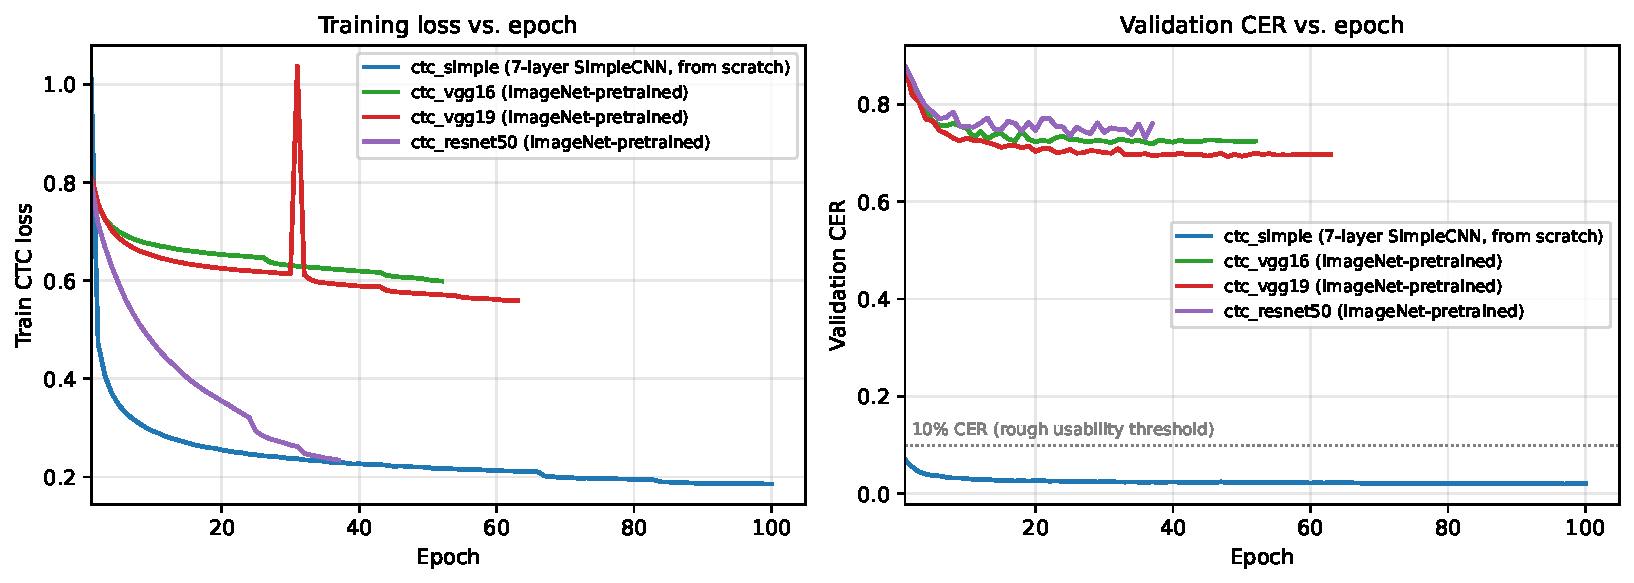
\includegraphics[width=\linewidth]{figures/training_curves.pdf}
\caption{Training dynamics of \texttt{ctc\_simple} (blue) vs.\ the ImageNet pretrained CTC variants \texttt{ctc\_vgg16} (green), \texttt{ctc\_vgg19} (red) and \texttt{ctc\_resnet50} (purple). Left: training CTC loss, \texttt{ctc\_simple} converges to near zero, the VGG pair underfits, ResNet50 overfits. Right: validation CER, \texttt{ctc\_simple} reaches below 10\% while all pretrained variants stay stuck around 0.70 until early stopping.}
\label{fig:training-curves}
\end{figure} 

\texttt{ReduceLROnPlateau} repeatedly halved the learning rate with no resulting improvement in validation CER for any of the failed variants. This behaviour rules out one obvious reason that learning rate was too high or of gradient instability, because both would normally respond to a smaller step size. The pretrained backbones were already updating at a very low effective learning rate (a base of $3{\times}10^{-5}$, further scaled by 0.1 on the backbone to give $3{\times}10^{-6}$), so too little learning might have been the issue. The VGG pair illustrates this, with training loss barely moving ($0.81 \rightarrow 0.60$), which is what one would expect if the backbone is learning too slowly to adapt. ResNet50 reveals something else. Training loss falls sharply from $0.80$ to $0.23$ over 37 epochs while validation CER stays flat. This indicates the head had enough  capacity to fit and memorise the pretrained features, but those features did not transfer to the character-level recognition task in the first place.

Concrete prediction examples for \texttt{ctc\_simple} on the in domain test-set are shown in Figure~\ref{fig:report-predictions}.
Full results comparison in Figure~\ref{fig:comparison1}. 
\begin{figure}[h]
\centering
\small
\begin{tabular}{p{0.93\linewidth}}
\toprule
\textbf{(a) Correct transcription (CER $=$ 0\%)} \\
\midrule

\includegraphics[width=\linewidth]{figures/correct1.jpg} \\
\textbf{Ground truth:} \textit{julev- ja davvis\'{a}migielagiiguin ja s\'{a}miiguin geat eai} \\
\textbf{Prediction:} \textit{julev- ja davvis\'{a}migielagiiguin ja s\'{a}miiguin geat eai} \\
\midrule
\textbf{(b) Diacritical error (CER $=$ 8.3\%)} \\
\midrule

\includegraphics[width=\linewidth]{figures/diacritical_errors_new.jpg} \\
\textbf{Ground truth:} \textit{ođđasis eal\'{a}skahttojuvvon) Suohkana h\'{a}lddahusla\v{s}} \\
\textbf{Prediction:} \textit{oddasis eal\'{a}skahttojuvvon) Duohkama h\'{a}lddahusla\v{s}} \\
\footnotesize \textit{Note: ođđasis $\rightarrow$ oddasis is the classic đ$\rightarrow$d error (the stroke is missed by the model).} \\
\midrule
\textbf{(c) Uppercase error (CER $=$ 29.6\%)} \\
\midrule

\includegraphics[width=\linewidth]{figures/uppercase_errors.jpg} \\
\textbf{Ground truth:} \textit{FYLKKAGIELDDAIGUIN. FINNM\'{A}RKKU FYLKKAGIELDDAS LEA \'{A}IGUMU\v{S}\v{S}IEHTADUS S\'{A}MI} \\
\textbf{Prediction:} \textit{FYLKKAGIELDDAIGUI0. F1O0m\'{A}RKKU FYLKKAGIELDDAs LEA \'{A}IGUmU\v{S}e} \\
\footnotesize \textit{Note: all uppercase lines are rare in the training distribution. The model frequently slips into mixed case or substitutes letters with visually similar digits.} \\
\bottomrule
\end{tabular}
\caption{CNN-CTC predictions illustrating the model predictions. (a) most lines are accurately transcribed, (b) diacritical strokes are the most common error, (c) all uppercase lines, rare in the training distribution, are by far the worst case.}
\label{fig:report-predictions}
\end{figure}

\begin{figure}[h]
\centering

\includegraphics[width=\linewidth]{figures/benchmark_comparison2.png}
\caption{Test set CER, WER, and exact match accuracy across 11 models (7 TrOCR variants, the lightweight CNN-CTC, and 3 failed ImageNet pretrained backbones). Lower values are better for CER and WER, higher values are better for exact match accuracy.}
\label{fig:comparison1}
\end{figure}

\section{Out of Domain Generalisation}
\label{sec:ood}

The out of domain evaluation on synthetic renderings of Turi's \turiYear{} \textit{Muitalus s\'{a}miid birra} produced rather surprising results. In domain, TrOCR has the best accuracy at \trocrSynthHFCER{}\% CER on the Spr\r{a}kbanken validation samples alone, against \ctcCER{}\% for \texttt{ctc\_simple}. 

On the historical text test set, TrOCR degrades by \trocrSynthDeltaCER{}~pp (\trocrSynthHFCER{}\% $\rightarrow$ \trocrSynthBookCER{}\%) while \texttt{ctc\_simple} is essentially flat (\ctcCER{}\% $\rightarrow$ \ctcBookCER{}\%). One TrOCR variant (\texttt{trocr\_smi\_pred\_synth}) still beats \texttt{ctc\_simple} on raw book CER (\trocrPredSynthBookCER{}\%). After punctuation and whitespace normalisation, however, the lightweight model overtakes all TrOCR variants on book text (\ctcBookNormAcc{}\% normalised accuracy vs.\ \trocrSynthBookNormAcc{}\% for the best TrOCR) (See Figure~\ref{fig:dataset-comparison}).

The sample is small (\bookTestSamples{} pairs) so it's nowhere near conclusive, but it might suggest that the smaller model learns more transferable character level features and is less prone to overfitting to synthetic rendering artefacts in the training distribution.


\begin{figure}[h]
\centering

\includegraphics[width=\linewidth]{figures/per_dataset_comparison.png}
\caption{Per Dataset Comparison: Spr\r{a}kbanken validation split vs Turi's \turiYear{} \textit{Muitalus s\'{a}miid birra} benchmark results.
Exact match accuracy on the book set is near zero for all models due to punctuation and orthography discrepancies. Normalised accuracy is the more informative metric here.}
\label{fig:dataset-comparison}
\end{figure}



\section{Conjunction Based Sentence Splitting}
\label{sec:conjunction-split}

Splitting long inputs at North S\'{a}mi conjunction boundaries before OCR and rejoining the predictions afterwards dropped long sentence CER from \splitLongOriginalCER{}\% to \splitLongSplitCER{}\%, a \splitImprovement{}pp improvement, below the short sentence baseline of \splitShortCER{}\% removing the length accuracy degradation (paired test $p = \splitPValue{}$, Cohen's $d = \splitCohensD{}$, \splitImproveRate{}\% of split samples improved, none degraded). Sentence length against CER and improvements visible in Figure~\ref{fig:cer-vs-length}.

% oracle upper bound
It is worth mentioning that the splitter acts on the ground truth strings rather than on a input OCR prediction, which makes the reported numbers a best case scenario, for the deployable variant would have to detect conjunctions on a noisy data (where short tokens like \textit{ja} and \textit{go} may themselves be misrecognised) or fall back to whitespace based segmentation of the line image, both of which are expected to lose much of the stated \splitImprovement{}\,pp gain. In addition, each segment is re-rendered as a fresh clean synthetic line image before OCR, so the experiment idealises both the segmentation \emph{and} the image quality, further inflating the reported upper bound.


\begin{figure}[h]
\centering
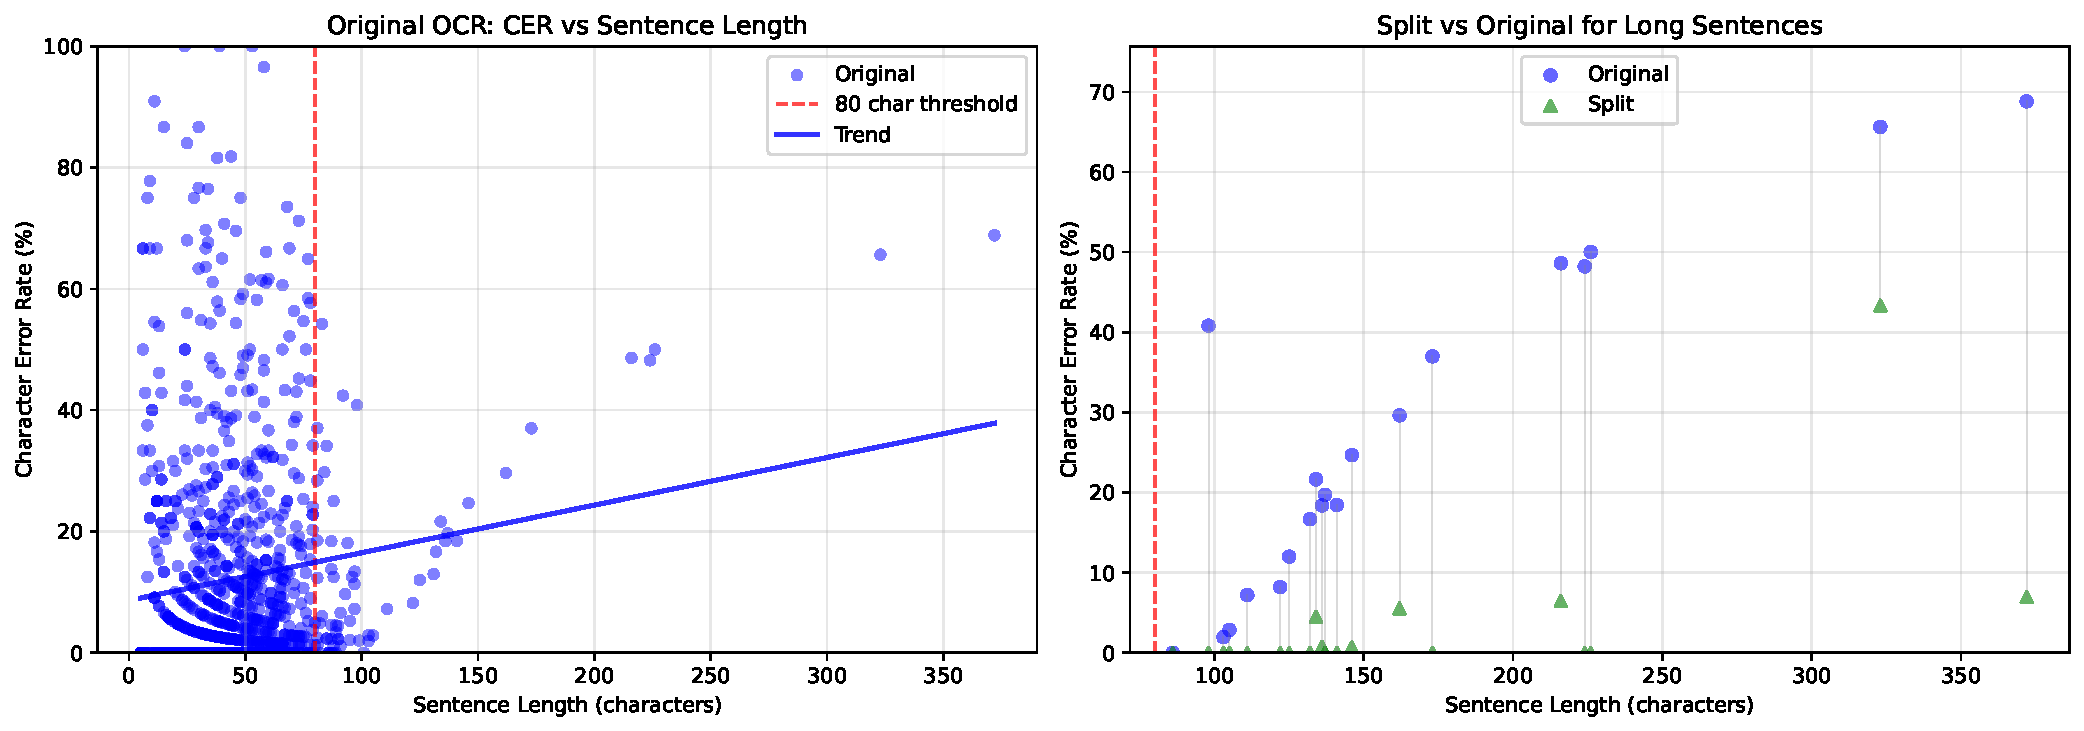
\includegraphics[width=\linewidth]{figures/cer_vs_length.pdf}
\caption{Character Error Rate of the lightweight CNN-CTC against the sentence length and the CER change after the split experiment.}
\label{fig:cer-vs-length}
\end{figure}


\section{End to End Pipeline}
\label{sec:e2e}

After passing the OCR predictions into TartuNLP's North S\'{a}mi English machine translation API~\cite{tartunlp}. The output scored BLEU \bleuScore{}, chrF \chrfScore{}~\cite{popovic2015chrf} and TER \terScore{}\% on the out of domain parallel set.

The moderate translation quality reflects how OCR errors propagate downstream, and the effect is even more pronounced for agglutinative languages. At \ctcCER{}\% CER, many of the relatively minor character errors land on the word endings that signal a noun's grammatical role or attach meaning like tense, number, and possession, rather than on the core part of the word that carries its meaning. Because these endings encode how words relate to one another in a sentence, a single dropped character can flip way the whole clause is read and degrade MT accuracy further. The results do not yield a fully fluent automatic translation, but they show that an end to end pipeline is in fact viable, even if for now it is best suited to simple downstream tasks such as archival indexing or content discovery rather than complete translation.


\begin{figure}[h]
\centering
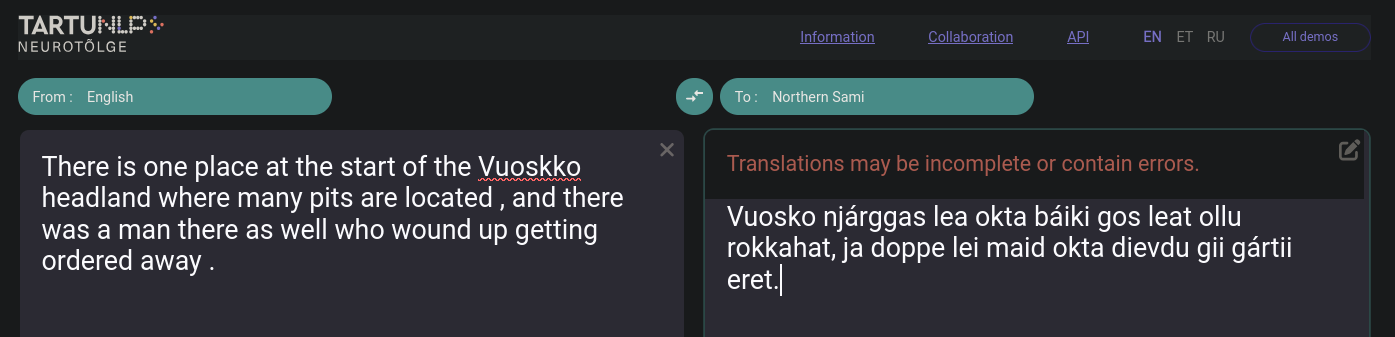
\includegraphics[width=\linewidth]{figures/tartu_nlp_translation.png}
\caption{The TartuNLP translation web interface, available at \protect\url{https://translate.ut.ee/}. The same backend is used programmatically in the end to end pipeline via TartuNLP API.}
\label{fig:tartu-nlp}
\end{figure}


\section{Applications}
\label{sec:applications}
The lighweight OCR models allows multiple application cases. The community driven preservation projects (small archives, local museums, language enthusiasts) typically operate without dedicated GPU or many resources at hand. A model that runs on a phone or a small laptop and fully offline, would remove the deployment friction that would otherwise keep these efforts away from being realized.  The lightweight model is realistic as the OCR layer in a search and indexing pipeline over million page historical corpora in archival context, or as a back-end for educational tools that need to react to text in real time (for example, mobile flashcards that take a photo of a S\'{a}mi book page). Lastly, a combination of the CNN-CTC model with a generative model (a Stable Diffusion inpainting pipeline) for joint recognition and reconstruction of occluded text. Figure~\ref{fig:report-applications} shows the proof of concept output, an artificially occluded North~S\'{a}mi line is fed through OCR and inpainting, producing both a transcription and a plausible reconstruction of the original image with damaged text. This kind of pipeline becomes possible only when each component is small and fast enough to run together on an embedded device, useful in self driving settings (partially obscured road signs), in retail (damaged product labels), or in next generation robotic assistants where text in the visual scene must be interpreted continuously.

\begin{figure}[h]
\centering
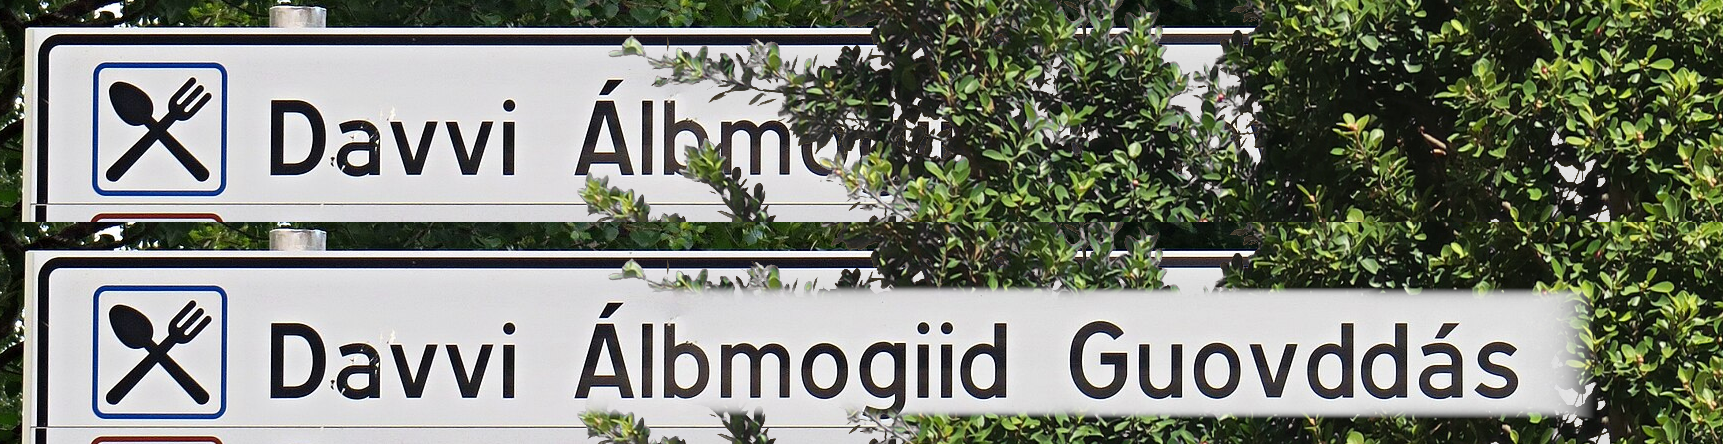
\includegraphics[width=\linewidth]{figures/reconstruction.png}
\caption{Proof of concept damaged text reconstruction combining \texttt{ctc\_simple} with a generative inpainting model on an artificially occluded North~S\'{a}mi line. The pipeline produces both a transcription and a reconstructed image. Enabled by the lightweight footprint, out of reach for the TrOCR baseline. Demonstrated as a future work direction in the IISA paper.}
\label{fig:report-applications}
\end{figure}

\section{Future work}
\label{sec:future-work}

The project leaves several questions unanswered and opens multiple options for future work. 
The main question still open to investigation is robustness to physical degradation. The entire benchmark in this thesis is conducted on synthetic renderings, and collecting and annotating a small corpus of real scanned S\'{a}mi documents (with realistic artefacts such as paper texture, ink bleed, skew and historical fonts) would validate the project's applicability.
The CTC model is weakest on rare inflected forms. Integrating Giellatekno's morphological analyser~\cite{moshagen2014} as a post correction layer, for instance by rescoring the top $k$ CTC hypotheses against a finite state lexicon, could selectively repair exactly the errors that propagate worst into downstream MT, without enlarging the deployed model.
Next, as \texttt{ctc\_simple} works on line level, applying Layout analysis and full page processing by pairing it with a lightweight line and region detector would elevate its usability from transcribing a cropped line to being able to process a full page, which matters for archival use cases.
Furthermore, it would be beneficial to check if the same approach works on different languages. Retraining the same architecture on other Uralic varieties (Inari, Skolt, Lule S\'{a}mi) or on unrelated low resource scripts would test if the same choices generalise, and if the same ImageNet pretraining issue appears. Finally, because the current decoder is purely greedy, showing the model's confidence in its predictions would increase the model's transparency.



\section{Conclusion}
\label{sec:conclusion}

The honest answer to the research question from (Section~\ref{sec:research-question}) is: \textbf{partially}. Depandant on the specific aspect of the question, the answer ranging from  yes to inconclusive.
\begin{itemize}
  \item \textbf{Deployment:} The size and speed advantage of \texttt{ctc\_simple} over the strongest TrOCR baseline is the difference between a million page archive processable in hours on widespread available hardware and one that would take days, and the difference between an OCR model that fits on a phone and one that does not. Unequivocally addressing the goal as achieved.
  \item \textbf{Accuracy:} On the in domain synthetic benchmark, \texttt{ctc\_simple} trails the best TrOCR variant by only \cerGap{}\,pp in CER, closer than the size difference would predict, and on the out of domain historical text subset it actually overtakes TrOCR on normalised accuracy. However, for an agglutinative language those few percentage points make a huge difference. The downstream OCR$\rightarrow$MT pipeline might be enough for archival indexing or content discovery but not for fluent automatic translation. Answering the question as yes but with few caveats.
  \item \textbf{Validation:} The entire evaluation in this thesis is conducted on synthetic renderings, with \bookTestSamples{} out of domain samples drawn from a single 1910 book. The model's behaviour on real scanned documents, with realistic paper, ink and degradation artefacts, has not been tested. As of now, the question remains unanswered.
\end{itemize}

The six contributions stated in Chapter~\ref{chap:goals} are all delivered: a lightweight CNN-CTC architecture, a systematic 11 model benchmark, a Sustainable AI footprint argument, an end to end OCR$\rightarrow$MT pipeline, a linguistically motivated conjunction splitting method, and a discussion of education, AI~\&~NLP and robotics applications. The three ImageNet pretrained CTC baselines did not converge, so the within CTC comparison is partial, the out of domain set is small, and no real scan data was used. 




\appendix

% Methodological background (CNN/VGG/ResNet/BiLSTM/Transformer/CTC primer)
\chapter{Background Concepts and Methods}
\label{appendix:concepts}

\section{Convolutional Neural Networks}
\label{sec:appendix-cnn}

A Convolutional Neural Network (CNN) is a deep learning architecture that processes images by sliding small, learned filters (kernels) across the input and stacking the resulting activations into feature maps.
The filters are shared across layers, which reduces the parameter count compared to a fully connected network of the same depth.
Stacking many convolutional layers lets the network learn a hierarchy of features: simple edges and textures in the early layers, character level structures in the deeper ones.

\paragraph{Feature maps.} Output of the convolutional layer. Each convolutional filter produces a feature map, it's a 2D array of activations indicating where in the image the pattern, the filter has learned (edges, corners, or a diacritical marks), is present. The set of input neurons that project to the same convolution neuron is called its \textit{receptive field}. As the network goes deeper, the receptive field grows, allowing later layers to capture larger spatial patterns. In OCR, this means that deeper layers can learn to recognise whole characters or character combinations, while early layers focus on local features like strokes and diacritics.

\paragraph{Activation Function}
After each convolution, a non linear activation function (ReLU in this case) is applied element wise to the feature maps. This allows the network to learn complex, non linear relationships between the input pixels and the output features.
ReLU (Rectified Linear Unit) is a common choice because it mitigates the vanishing gradient problem and promotes sparse activations, which can improve learning efficiency.

\paragraph{Subsampling (Pooling).} Pooling layers downsample feature maps, typically by taking the maximum (max pooling) or average activation value over a small spatial window. They make the representation more compact, enlarge the receptive field of subsequent layers, highlight the most important features, and introduce a small amount of translation tolerance.

\paragraph{Column features (adaptive pooling).} For OCR, the 2D feature maps produced by the CNN must be reshaped into a 1D sequence that downstream sequence models (BiLSTM, Transformer, CTC) can consume. \textit{Adaptive pooling} collapses the vertical axis to height 1, leaving a sequence of column vectors that runs left to right across the image. Each column vector summarises a thin vertical strip of the original image and is treated as one ``timestep'' by the encoder. This trick is what lets a fundamentally 2D convolutional model emit a sequence amenable to CTC.

\section{VGG16 / VGG19}
\label{sec:appendix-vgg}

VGGNets~\cite{simonyan2015vgg} are a family of deep CNNs, developed by Visual Geometry Group (VGG) which showed that by simply adding more layers (depth), the accuracy of image classification can improve. By  stacking many small 3$\times$3 convolutions, VGG16 and VGG19 (16 and 19 weight layers respectively) became standard pretrained backbones because of their simple, uniform structure.

\section{ResNet50 / ResNet101}
\label{sec:appendix-resnet}

ResNet~\cite{he2016resnet} introduced residual "skip" connections that let each layer learn a correction to the identity mapping rather than a full transformation. This enables stable training of much deeper networks. ResNet50 and ResNet101 have 50 and 101 weight layers respectively, avoiding the gradient vanishing problems that occur in very deep CNNs.

\section{ImageNet Pretraining and Transfer Learning}
\label{sec:appendix-pretraining}

The VGG and ResNet backbones used in this pipeline ship with \textit{ImageNet pretrained} weights, meaning they have already been trained on the ImageNet ILSVRC subset (~1.28M images across 1000 categories) that torchvision uses for its pretrained classification models. \textit{Transfer learning} reuses these weights as initialisation for a different downstream task. Like here, for OCR on North S\'{a}mi line images.

\section{BiLSTM}
\label{sec:appendix-bilstm}

A bidirectional Long Short Term Memory (BiLSTM)~\cite{hochreiter1997lstm} network is a type of Recurrent Neural Network (RNN) that runs two LSTMs over the column features, one left to right, the other right to left, and concatenates their hidden states at each position.
The RNN is a type of neural network for sequential data processing. They have a hidden state that is updated at each timestep based on the current input and the previous hidden state, allowing them to capture temporal dependencies. However, normal RNNs suffer from the vanishing gradient problem, which makes it difficult to learn long range dependencies.
The LSTM cell uses learned input, forget, and output gates to retain long range dependencies while suppressing irrelevant context, mitigating the vanishing gradient problem, which is well suited to OCR: predicting the character in a column often benefits from knowing both what came before and what is coming next, for example to disambiguate visually similar diacritics by their typical neighbouring characters in S\'{a}mi morphology.

\section{Transformer Encoder}
\label{sec:appendix-transformer}

A Transformer encoder~\cite{vaswani2017attention} replaces recurrence with self attention: every position attends to every other position in parallel, weighted by learned compatibility scores. This gives a fully global receptive field over the column features and removes the sequential bottleneck of recurrent models.
In the pipeline, the Transformer encoder serves as a drop in alternative to the BiLSTM, isolating whether explicit global attention buys more than the LSTM's local bidirectional context for the relatively short column sequences produced by the backbone.

\section{TrOCR}
\label{sec:appendix-trocr}

TrOCR~\cite{li2023trocr} is a transformer based OCR architecture using a Vision Transformer (ViT) encoder paired with an autoregressive text generation decoder. Rather than treating the image as a sequence of column features (the CRNN approach used by this pipeline), TrOCR splits the image into a grid of fixed size patches and processes them with self attention end to end. The decoder then generates output text token by token, conditioned on the encoded image and on its own previous outputs.

\section{Connectionist Temporal Classification (CTC)}
\label{sec:appendix-ctc}

Connectionist Temporal Classification (CTC)~\cite{graves2006ctc} is a loss function and decoding scheme for sequence labelling tasks in which the alignment between input frames and output labels is unknown. CTC introduces a special \textit{blank} token and marginalises over all alignments that, after collapsing repeated tokens and removing blanks, produce the target transcription. This removes the need for explicit character level segmentation of the input image, exactly the property needed for variable length OCR lines. At inference time, greedy decoding picks the most likely token at each timestep and applies the same collapse rule to produce the final transcription.

\section{AdamW Optimizer}
\label{sec:appendix-adamw}

AdamW is the optimiser used across all training runs in this pipeline. Adam, the underlying algorithm, adapts the per parameter learning rate using running averages of recent gradients (a momentum term) and their squared magnitudes (a scale term). This makes it robust on noisy gradients and forgiving of poor initialisation, which is why it has become the de facto default for modern deep learning. The ``W'' variant detaches the weight decay from the adaptive scaling.

\section{Learning Rate (LR), LR Schedulers and Weight Decay}
\label{sec:appendix-lr}

The \textit{learning rate} controls the step size taken along the gradient direction when updating weights of the model.

\paragraph{Differential learning rates.} Apply different LR multipliers to different parameter groups inside the same optimiser.

\paragraph{LR schedulers.} Change the learning rate over the course of training.

\texttt{ReduceLROnPlateau}, monitors the validation CER and halves the learning rate whenever it stops improving for a fixed number of epochs, so the network starts in an aggressive regime and gradually settles into a finer grained one without manual intervention. \textit{Warmup} works at the other end of training: starting from a tiny learning rate and ramping up over the first few epochs, which prevents large early gradients from destabilising pretrained weights.

\paragraph{Weight decay.} A regulariser that adds a small penalty proportional to the squared magnitude of each weight, gently pulling the network toward simpler solutions. This discourages overfitting and keeps unused weights from drifting to large arbitrary values that do not help generalisation.

\paragraph{Gradient clipping.} Caps the global norm of the gradient vector at a fixed threshold. 
CTC losses are prone to occasional spikes when the model is briefly very wrong about an alignment. Clipping it stops a single bad batch from blowing up the weights.

\section{Epochs, Batch Size, Training Steps, and Early Stopping}
\label{sec:appendix-training-loop}

An \textit{epoch} is one complete pass over the training set. The \textit{batch size} is the number of samples whose gradients are averaged before each weight update.
A \textit{training step} is a single weight update, one batch processed. The number of steps per epoch is therefore the dataset size divided by the batch size.

\textit{Early stopping} halts training when the validation metric has stopped improving for \texttt{patience} epochs, restoring the model from the best checkpoint observed.

\section{Data Augmentation}
\label{sec:appendix-augmentation}

Data augmentation expands the effective training set by applying random transformations to each sample on the fly: minor rotations, scale jitter, brightness and contrast perturbations, Gaussian blur, and synthetic noise. That way we can synthetically generate a more diverse set of training images.


\section{OCR Evaluation Metrics}
\label{sec:appendix-ocr-metrics}

OCR quality is measured against a reference transcription using string edit metrics. The \textit{Levenshtein distance} between two strings is the minimum number of single character insertions, deletions, or substitutions needed to turn one into the other.

\paragraph{Character Error Rate (CER).} The Levenshtein distance between the predicted and reference strings, divided by the length of the reference in characters. The lower the better.

% A CER of 0\% is perfect; values above 100\% are possible when the prediction is much longer than the target. CER is the headline metric throughout this report.

\paragraph{Word Error Rate (WER).} The same idea but at the word level: edit distance counted in word tokens rather than characters, divided by the reference length in words. WER is harsher than CER, because a single misrecognised character can corrupt an entire word.

\paragraph{Exact Match Accuracy.} The fraction of test samples for which the predicted transcription matches the reference verbatim. A binary, precision metric.

\paragraph{Normalised Accuracy.} Exact match accuracy computed after a normalisation pass (removing punctuation, collapsing repeated whitespace). Useful for separating substantive recognition errors from cosmetic formatting differences.

\section{Machine Translation Metrics}
\label{sec:appendix-mt-metrics}

\paragraph{n gram.} A contiguous sequence of n tokens. For example, in the sentence ``the cat sat'', the 1 grams are ``the'', ``cat'', and ``sat'', while the 2 grams are ``the cat'' and ``cat sat''. MT metrics often operate on n grams to measure how well the candidate translation matches the reference.

\paragraph{BLEU.} Bilingual Evaluation Understudy. Measures the n gram precision of the candidate translation against one or more references, multiplied by a brevity penalty that discourages overly short outputs. Widely used. Might be coarse for morphologically rich languages where surface forms vary heavily.

\paragraph{chrF.} Character n gram F score~\cite{popovic2015chrf}. Operates on character n grams instead of word n grams, which makes it more forgiving of morphological variation.

\paragraph{TER.} Translation Edit Rate: the number of edits (insertions, deletions, substitutions, shifts) needed to turn the candidate into the reference, normalised by the reference length. Closer to zero is better.

\section{Statistical Significance and Effect Size}
\label{sec:appendix-statistics}


\paragraph{Percentage points (pp).} The arithmetic difference between two percentage values, distinct from a relative percentage change.

\paragraph{Paired t test.} A hypothesis test for whether the mean difference between two paired sets of observations is zero. ``Paired'' means each prediction in condition A has a one to one counterpart in condition B.

\paragraph{p value.} The probability of observing a result at least as extreme as the measured one if the null hypothesis (no true difference) were true. A small p value (conventionally $p < 0.05$) is read as evidence against the null.

\paragraph{Effect size.} A standardised measure of \emph{how large} a difference between two conditions is, independent of sample size. A p value can be tiny merely because the sample is large, even if the underlying effect is negligible, effect sizes report the gap on a scale that is interpretable in its own right.

\paragraph{Cohen's $d$.} A common effect size statistic for the difference between two means: the mean difference between two conditions divided by the pooled standard deviation. It expresses the gap in units of typical variability, so it is comparable across studies and immune to sample size inflation. Conventional rules of thumb: $d \approx 0.2$ small, $0.5$ medium, $0.8$ large.

% Deliverables: code, models, conference submissions, supervision log
\chapter{Appendix}
\label{appendix:deliverables}

\section{Code and Models}
\label{sec:appendix-code}

\begin{enumerate}
  \item Source code (GitHub): \url{https://github.com/magwrap/north-sami-ocr/}
  \item Trained lightweight CNN-CTC model card (HuggingFace): \url{https://huggingface.co/magwrap/cnn-ctc-ocr-sme}
  \item Spr\r{a}kbanken synthetic S\'{a}mi OCR dataset (HuggingFace, mirrored): \url{https://huggingface.co/datasets/magwrap/synthetic_sami_ocr_data}
\end{enumerate}


\section{Conference Submissions}
\label{sec:appendix-submissions}

\begin{enumerate}
  \item \textbf{IISA 2026}, International Conference on Information, Intelligence, Systems and Applications. Full paper accepted to the \textit{21st century AI and education} theme. Venue: \url{https://easyconferences.eu/iisa2026/}.
  \item \textbf{SCAI 2026}, 15th Scandinavian Conference on Artificial Intelligence. Extended abstract accepted to the \textit{AI for Good: Innovation, Ethics, Society} theme. Venue: \url{https://www.sdu.dk/en/forskning/sdu_applied_ai_and_data_science/scai}.
\end{enumerate}

\section{Supervisor and Meeting Log}
\label{sec:appendix-supervision}

Weekly meetings were held on Tuesdays, serving as the primary supervisory mechanism throughout the project. These meetings provided a structured opportunity for regular check ins, progress updates, and feedback sessions. The discussions during these meetings were instrumental in guiding the research direction, troubleshooting issues, and refining methodologies.

\section{AI usage}

This declaration follows SDU's guidelines on generative AI in student work, which require transparent disclosure of how AI contributed to the final product. Throughout the project, generative AI tools, namely Claude Code (Sonnet 4.6, Opus 4.7, Opus 4.8) were utilized for the following categories of tasks:
\begin{itemize}
  \item \textbf{Programming and code generation}: AI assisted with writing code snippets, boilerplate, and data processing scripts. Example: the alignment tool experiment for parallel corpora, which would normally require weeks of development time, was prototyped in hours with AI assistance, freeing time for experimentation and analysis. All AI-generated code was read, tested, and modified before integration.
  \item \textbf{Brainstorming and ideation}: AI was used to generate ideas, suggest alternative approaches, and surface considerations that a less experienced researcher might overlook. All directions explored were subsequently verified against the literature and the supervisor's feedback.
  \item \textbf{Language proofreading}: AI was used to check grammar, spelling, punctuation, and to improve clarity of phrasing. AI-suggested rewordings were reviewed and edited before integration.
  \item \textbf{Structure and organization}: AI was occasionally consulted on chapter and section ordering and on how to frame arguments. 
  \item \textbf{Figure generation}: AI assisted in producing the Python/matplotlib scripts used to generate figures and LaTeX tables (see \texttt{figures/scripts/}). The underlying data and the analytical claims drawn from there were independent of AI.
\end{itemize}

\noindent\textbf{Transparency and accountability.} No AI-generated text or output is presented in this report as the my own work without disclosure. I have critically evaluated every AI contribution for relevance, accuracy, and factual correctness, and take full responsibility for the final content of the report.

\bibliographystyle{unsrt}
\bibliography{mybibliography}

\end{document}
